\chapter{Calorimetry}
\label{Chapter:Calorimetry}

\section{Introduction to calorimeters}
\label{sec:intro}
%
Calorimeters of the CEPC detector, including electromagnetic calorimeter (ECAL) and hadron calorimeter (HCAL), are employed for precise energy measurements of electron, photon, tau and hadronic jets. To fully exploit the physics potential about Higgs, W, Z and related SM processes, the jet energy resolution $\sigma_{E}/E$ is required to reach 3\%-4\%, or $30\%/\sqrt{E}$ at energies below about 100~GeV. This resolution is about a factor of two smaller than the calorimeters used for the LEP detectors and currently operating calorimeters at the LHC. It significantly improves the separation of the W and Z bosons which decay into two jets, as shown in Figure~\ref{fig:cal-WZ}. The basic requirements for ECAL and HCAL resolution are $16\%/\sqrt{E}$ and $50\%/\sqrt{E}$, respectively.\\
%
\begin{figure}[tbp]
\centering
\includegraphics[width=14.cm]{Figures/Calorimetry/cal-WZ-separation.jpg}
\caption{\label{fig:cal-WZ} Separation of W and Z bosons with different jet energy resolutions.}
\end{figure}
%

To achieve the required jet energy resolution, many R\&D researches are carried out within the CALICE collaboration since 2000~\cite{calice}. The majority of these studies aim to develop extremely fine granularity and compact imaging calorimeters with several technology options shown in Figure~\ref{fig:cal-PFA}. Imaging calorimeter is a rapidly developing novel particle detector which has excellent spatial resolution. It is capable to provide enormous position information of incident and showering particles, which makes it possible to reconstruct every single particle cluster. This is vital for Particle Flow Algorithm (PFA~\cite{cha411}) and help to significantly improve the energy resolution of hadrons. The basic idea of PFA is to distinguish charged ($\sim$65\%) and neutral particles ($\sim$35\%) inside the calorimeters. Charged particles measured in the inner tracker with high momentum resolution are matched to their energy depositions in the calorimeters. Energy depositions without matched inner tracks are considered to originate from neutral particles inside jets, among these neutral particles, about 25\% of energy from photons are measured in the ECAL with good energy resolution, while the residual energy of merely 10\% from neutral hadrons are measured by the calorimeters with poor energy resolution. Hence, the jet energy is determined by the charged track momenta of charged particles from inner tracker and energy depositions of neutral particles in the calorimeters. It has been demonstrated that significant improvement of the jet energy resolution is achievable based on MC simulations and test beam measurements. However, more efforts are needed to optimize the calorimeter design, to improve the PFA, and
to develop the technologies for high granularity imaging calorimeters.\\

%
\begin{figure}[tbp]
\centering
\includegraphics[width=14.cm]{Figures/Calorimetry/cal-PFA.jpg}
\caption{\label{fig:cal-PFA} PFA: Imaging calorimeters being developed by the CALICE collaboration since 2000.}
\end{figure}
%

The calorimeter system includes two sub-detectors, an electromagnetic calorimeter (ECAL) which is optimized for the
measurement of photons and electrons, and a hadronic calorimeter (HCAL) which is employed to measure the energy
deposit of the hadronic showers caused by the hadronic particles when they are absorbed in the HCAL detector. The
two sub-detectors will be installed within the solenoid to minimize the inactive material in front of the calorimeters
and to reliably associate tracks to energy deposits. The calorimeter system is divided into three parts, one cylindrical
barrel and two end-caps.

The ECAL consists of layers of active sensors (such as silicon pads or pixels, or scintillator detector) interleaved
with absorber tungsten plates. The digital HCAL (DHCAL) is expected to have stainless steel absorber plates with gaseous detectors
such as glass Resistive Plate Chambers (gRPC) or GEM, or analog HCAL (AHCAL) using scintillator with SiPM readout as sensor.
Both ECAL and HCAL are sampling detectors with very fine granularity and segmentations of electronic readout
which is driven by excellent separations requirement between charged and neutral particles for the particle flow algorithms.

From Figure~\ref{fig:cal-PFA}, there are more detector options with enormous worldwide R\&D efforts ongoing within the
CALICE collaboration.
Another approach for high performance calorimeters is dual-readout calorimetry.

However, for this particular CDR, we have to be selective and focus on a few options with collaborators
who expressed great interests so far. The CEPC detectors R\&D is widely open for international
collaboration with different detector options and new ideas.

%%%%\\\\\\\\\\\\\\
\section{Electromagnetic Calorimeter for Particle Flow Approach}
%
The particle flow paradigm has tremendous impact on the design of the electromagnetic calorimeter detector. Separating overlap showers from each other is principal requirement of the detector. A calorimeter used for particle flow thus needs to be able to do pattern recognition in the shower. The electromagnetic section has lots of tasks to fulfill. It should be able to select photons from close-by particles. It should be able to reconstruct the detailed properties of the shower, such as shower shape, starting point and energy distribution. It should be able to distinguish early starting electromagnetic showers from hadronic ones. The imaging capabilities of the calorimeter are more important than the intrinsic single particle energy resolution, although the latter is still important to the particle flow performance for electron, photons and jets. Due to the reason that about half of the hadronic showers will start development inside the electromagnetic calorimeter, a calorimeter with excellent three dimensional granularity is of utmost importance. In order to have the ability of separate close-by showers in the calorimeter, the detector with small Moliere radius is required. A large ratio between interaction length and radiation length of the detector is advantageous to the separation between electromagnetic and hadronic showers. A small radiation length will make the start of the electromagnetic shower earlier in the calorimeter, while a large interaction length will reduce the fraction of hadronic showers starting in the calorimeter. At the same time, the calorimeter with a compact structure is favorable.\\

In this section, we focus on two detector options for the ECAL, which consist of layers of active sensors (silicon pads or pixels, or scintillator detector) interleaved with absorber tungsten plates.


\subsection{Silicon-Tungsten Sandwich Electromagnetic Calorimeter}
\subsubsection{Introduction}

The study of the Higgs is not the only goal of a machine at 250 centre-of-mass
energy. It can be generalised to the multi boson physics (Z, W and H). The best
way to use the excellent luminosity foreseen at CEPC, consist to tag the boson
through their mass in their decays into $q\bar{q}$ (2 jets). Taking into account
the natural width of the Z and W, it has been shown that this goal required to
achieve a jet energy resolution of $30\%/\sqrt{E_\mathrm{Jet}}$, thus a factor
two better than the energy resolution achieved for a typical detector at LEP.

It has been shown~\cite{Videau:2002sk} that a method consisting to fully
reconstruct every single particle could reach this goal (Particle Flow
Algorithm); it requires both a high performance tracker, typically achieving
$\delta p / p$ of $10^{_5} p / GeV$ associated with high granularity
calorimeters able to separate the contribution from individual particles down to
the MIP level. %
As a typical jet is contains fractions in energy of 65\%, 25\% and 10\% of
charged particles, photons and neutral hadrons respectively, a moderate
calorimetric resolution is then sufficient to achieve the goal. %
In this framework, the electromagnetic calorimeter (ECal), is first devoted to
measure photon(s) and to a lesser extent electron(s) and to make a full pattern
of the deposited energy of the hadron, i.e. shower of hadron interacting in the
ECAL. %
To avoid ``blind region'', the entire calorimeter has to be put inside the
super-conductive solenoid. The compactness is therefore an important criterion.

The design of the calorimeters have to take the following guidelines into
account~\cite{Videau:2002qf}:
\begin{itemize}
\item Optimisation of the number of calorimeter cells (cell size and number of
  layers)
\item Choice of the absorber material in order to insure a high level of
  compactness and the infra-structural components such as cooling, power
  supplies, readout cables and the very front end electronics.
\end{itemize}
For the electromagnetic calorimeter these criteria has led to the choice of
Tungsten with a radiation length of Xo=3.5{mm}, a Moli�re radius of
RM=9{mm} and an interaction length of $\lambda_\mathrm{I}=96{mm}$.

\subsubsection{Silicon sensors}
\label{sec:SiW-Si}

Among several sensor techniques, high resistivity silicon pin diodes offer
several unique intrinsic advantages:
\begin{itemize}
\item stability: under a reasonable bias voltage, completely depleted pin-diode
  have a gain of one, and a signal response to MIP mostly defined by the
  thickness of the sensor, with a very low dependence on temperature, radiation,
  humidity, ...
\item uniformity: for the same reason, the control of the thickness over large
  batches (typically to less than a percent) ensures a uniformity of response
  within a wafer and between them. %
  The nonsensitive area between wafers has recently been reduced by the use of
  laser cutting, thinned guard-ring design~\cite{Cornat:2009zz}, and would
  benefit from the use of larger ingot size (8'' becoming the standard).
\item flexibility: the dimension and geometry of the cells are defined by the
  readout pad on the PCB.
\item High Signal-to-Noise ratio: with $\simeq80$ electron-hole pairs created by
  linear mm of MIP track, MIPs tracks can easily be traced in the calorimeters,
  which is critical for the god performance of
\end{itemize}
The only real drawback of Silicon sensors remaining is their price, to be
expected around $2-3{\$/cm^2}$.

By associating of Silicon sensors with Tungsten absorbers and Carbon Fibre
structures, the SiW-ECAL offers an excellent option for PFA optimised
calorimetry.

\subsubsection{Constraints}
\label{sec:SiW-Constraints}

High granularity calorimetry, and ECal especially, is technically challenging:
the very number of channels calls for an embedded readout and zero suppression,
to limits the amount of connections; in turn embedded readout power consumption
should be as limited as possible to avoid large cooling systems which would
degrade the capacity of the calorimeter. In the best case the cooling should
stay passive at the heart of the calorimeters.

The design proposed for the CEPC SiW-ECal is very largely inspired by the one of
the ILD detector for ILC as described in the Detector baseline
Document~\cite{ILD_DBD:2013}; it is influenced by the options studied for the
CMS High-Luminosity upgrade endcap replacement HGCAL~\cite{Magnan:2017exp,
  Martelli:2017qbe}, concerning cooling and electronics. In terms of luminosity
and collision rates, the CEPC lies between the 2 options.

\subsubsection{Mechanics \& design}
\label{sec:SiW-Design}

The geometry presented here reflects the current (october 2017) status on the
realistic models developed for ILD. It differs slightly form the CEPC\_v1 and
CEPC\_v4 models~\cite{Zhao:2017}, mainly on ECAL thickness ($223{mm}$ vs
$185{mm}$), and inner radius of the endcaps ($226.8$ and $245{mm}$ vs
$400{mm}$).

% CEPCv1
% Barrel R = 1843-2028 mm (thickness = 185mm)
% Endcaps Z = 2450-2635mm (thickness = 185mm) ==> L = 4900mm
% Endcaps Rin = 226.8mm
% Cell_size = 5.0833mm
% HCAL Barrel Rin = 2058mm; Gap ECAL-HCAL = 30mm
% HCAL Endcaps Zin = 2650mm; Gap ECAL-HCAL = 15mm

% CEPCv4
% EndCaps Rin = 245mm
% Cell_size = 10.1667mm

\subsubsection{Geometry}
\label{sec:SiW-Geom}

The geometry of the detector is based on ILD detector, where there is no blind
zone between modules, but only ``special zone'', where it has been shown that
performance of the reconstruction of jets or photon(s) is not downgraded
significantly~\cite{Jeans:2017}. \\
The figure below shows this octagonal geometry and the possible way to build the
detector:
\begin{figure}[tbp]
\centering
\includegraphics[scale=0.6] {Figures/Calorimetry/SiW_ECAL_EndCaps.png}
\includegraphics[scale=0.6] {Figures/Calorimetry/SiW-Barrel.png}
\includegraphics[scale=0.2] {Figures/Calorimetry/SiW-ECAL-Barrel_module.png}
\caption{
  Left: Geometry of the SiW-ECAL Endcaps. %
  Middle: Barrel %
  Right: Geometry of the barrel modules. %
}
\label{fig:Siw_ECAL-geom}
\end{figure}

\paragraph{ECal thickness}

% VBTD: TO BE RECALCULATED WITH CEPC MODULES, IF COOLING...
For a baseline design featuring 30 layers -- split in 2 sections of 20 and 10
layers, holding each an equal amount of $12 Xo$ of W -- $525 microns$ thick wafers,
and a base plate of $20{mm}$ of carbon, the ECal thickness is estimated at
$223??{mm}$.

For a reduced number of layers, at 22 (with section of 14 and 8), but thicker
wafers ($725 microns$), the thickness becomes $191??{mm}$.

\paragraph{ECal dimensions}

% Dimension of small ILD as of Sept. 2017.

The Barrel consist of 8 staves of 5 trapezoidal modules. %
Each barrel module contains 5?? columns of alveoli. %
The number of modules and alveoli is even in order to avoid any special region
at the azimuthal angle $theta=0$. %
%VBTD Check coordinate system in global document
The alveolus size is fixed to $186 {mm}$ by mechanical limits and by cost
optimisation considerations, to contain exactly two 6-inch wafers or
one-and-a-half 8-inch wafer. %
Integrating the alveolus size, walls of modules and contingencies, the barrel
length amount to $4700 {mm}$. ($4900{mm}$ in CEPC simulations). %
A gap of typically $70 {mm}$ ($100{mm}$ in simulation) is left between the
barrel sides and end-cap front parts, whose precise dimension will depend on the
amount of ancillaries needed to service the ECAL and trackers (power and DAQ
cables, cooling pipes, patch panels).

The end-caps are made of quadrants of 2 modules of 4 and 3 alveoli columns.  %
Their inner radius is fixed by the ECal ring at $400{mm}$. %
With 7 alveoli columns, the end-cap outer radius is $1755 {mm}$. %
An overshoot of $32 {mm}$ is left between the outer radius of the barrel and
of the end-caps, in order to contain the EM shower impinging the region of
overlap. see figure~\ref{fig:SiW-ECAL_PhiScan}. %
This fixes the inner radius size of the ECal barrel at $1498 {mm}$ or
$1530{mm}$. %

\begin{figure}[tbp]
\centering
\includegraphics[scale=0.50] {Figures/Calorimetry/SiW_ECAL_X0_PhiScan.png}
\includegraphics[scale=0.70] {Figures/Calorimetry/SiW-ECAL_Theta_Scan.png}
\caption{ %
  Left: Thickness of Tungsten seen as function of the polar azimuthal angle scan
  of one octant of the barrel.  %
  Right: Mean Theta angle scan }
\label{fig:SiW-ECAL_PhiScan}
\end{figure}

For such a geometry, % C-x * d command for emacs-calc embedded
% [calc-mode: justify: left]
% [calc-mode: language: normal]
% cols := 8*5*5 + 2*4*7 =>
% slabsS := cols * 22 =>
% slabsL := cols * 30 =>
summing the barrel (200) and end-caps (56), 256 alveoli columns are needed.  %
For 22 (resp. 30) layers, and this yields 5632 (7680) alveoli, and as many
detector slabs.

\paragraph{Slab geometry}
In each alveola of the modules, a slab is inserted.  %
Slabs contains 2 symmetric layers of Silicon sensors glued on PCB, equipped
with readout ASICs, high voltage distribution by a Capton foil and copper layers
for passive cooling. %
The elements are chained on both sides of a Carbon fibre cradle taking the shape
of an H, with a core of Tungsten, and shielded by an aluminium cover. %
This so-called H-Structure is illustrated below.
\begin{figure}[tbp]
\centering
\includegraphics[scale=0.8] {Figures/Calorimetry/SiW-ECAL-Alveola_cut_525.png}
\includegraphics[scale=0.8] {Figures/Calorimetry/SiW-ECAL-Long_SLAB_eclate_sign_v2.png}
\caption{ %
  Left: Transverse cut through of a thin layer of the SLAB. %
  Right: Exploded view of the top layer of a slab of the SiW-ECAL. %
  The same structure is mirrored below the slab.  %
}
\label{fig:Siw_ECAL-Slab}
\end{figure}

To insure scalability and industrial production, the design has been made as
modular as possible: the basic unit is the ASU (Assembly Single Unit), made of a
$18�18{mm�}$ PCB onto which 4 wafers of $90�90{mm�}$ wafers are glued.  %
Each ASU would handle 256 cells with 4 ASICs, for cell surfaces of %
% 180 / 16 => 11.25
$11.25�11.25{mm�}$.

The ASUs are chained together for the clock and configuration distribution and
data collection. %
For a radius of %RinnerB%
$1498{mm}$ the longest (shortest) barrel slabs
measure %RinnerB * 2 * sin (Pi/8)
$1146{mm}$ ($955{mm}$). % short = long - ECAL thickness
In the end-caps, these number are ??, ??.

%In total ?? (?? )ASUs, ?? (??) {m�} of silicon, ?? (??) chips and ?? (??)
%ASICs assuming 64 channels per chip must be produced.

\subsubsection{Electronics}

One of the most critical element of the CEPC calorimeters is the readout
electronics which is defined by the dynamic range, the effective digitisation,
mode of trigger, the rate of working and power consumption per channel.

%\subsubsection{Dynamic range}
%\label{sec:SiW-DynRange}

{\bf {Dynamic range:}} A MIP going through a 725{$microns$} diode would produce % 80 * 750 = 60000
$\simeq 60000 $ electron-pairs holes or % * 1.6e-19 = 9.6 e-15
a charge of $9.6{fC}$?? as the most probable value (MPV). %
To record MIPs with an efficiency higher than 95\% this ports the low-end of the
dynamic range to a 1/3 of the MPV.  %
The high-end is determined by the number of MIP equivalent at the core of the
high-energy EM showers, which can reach up-to 10000 MPV or $96{pC}$ for
$11�11{mm�}$ cells. %
%If the typical precision aimed at for the calibration using MIPs is of the
%percent, one should expect 20-100 adcc at the MPV and
% VBTD: TO BE X_CHECKED
%full digital dynamic range of $10^6$, or 18-20 bits (maybe reduced to 16 using
%multiple dynamic ranges).

%\subsubsection{Timing}
%\label{sec:SiW_ECAL_timing}

{\bf {Timing:}} Time measurement of deposits in the calorimeters can be useful to Particle Flow
algorithms to help disambiguate particle contributions.  For the CMS HGCAL it is
planned to distinguish particle stemming from different
interactions~\cite{Magnan:2017exp}, by achieving a timing of $50-20{ps}$ on
EM showers.  %
For $e^+e^-$ colliders, with a single primary vertex, precision timing of
individual cells -- or group of cells -- could still be useful to reduced the
confusion and improve the resolution.  The required precision is uncertain and
should be studied further. %
Recent version of the SKYROC2a ASIC, could be operated~\cite{Suehara:2017} on
test board with a measure of time close to 1.4{ns}.  The performance has to be
measured in an integrated design. %

%\subsubsection{Rates}

%As a circular collider, the CEPC will run continuously with 2 bunches separated
%by $3.6??\u{\us}$ at the highest energy and ?? bunches separated by $??\u{\us}$
%in the high luminosity run.  %

{\bf {Rates:}} The running conditions a circular collider preclude any pulsed operation as is
planned for the linear ones, where clocks, pre-amps, digital conversion are
powered sequentially at a few Hz. %
A partial in-time shut-off or local on-demand switch-on of the ADC and TDC parts
can be envisaged, leaving the pre-amp as the single major power consumer.
% VBTD: check number for Klaus chip
% VBTD: to discuss with Stephane
As a point of reference, the current power consumption for SKIROC2 chips
designed for the SiW-ECAL of ILD is of $5{mW}$ per channel in continuous mode.


%\subsubsection{Occupancy}
%\label{sec:SiW-Occupancy}

{\bf {Occupancy:}} The occupancy of the calorimeters should be very low.
% VBTD NUMBERS, NUMBERS, NUMBERS!!!
This pushes in the the direction of designing pre-amps with a very small
consumption when there is no signal.



%\subsubsection{Ancillaries}

\subsubsection{Power \& Cooling}
\label{sec:SiW-Power}

To the first order, the amount of power dissipates scales with the number of
electronics channels.  One important issue is to decide on the power scheme:
\begin{itemize}
\item a reduced number of channels using only passive cooling at the heart of
  the detector, such as planned at the ILD; a $400{microns}$-thick copper sheet
  will drain the heat to the end of the slab, where it is removed by a cooling
  system.
\item keep a high granularity but include $\mathrm{CO}_2$ cooling in the
  absorbers such as envisaged for the HGCAL.
\end{itemize}

The CEPC ECAL is at edge of both options, with a limit for the purely passive
option of the order of $2�2{cm�}$ cells for a increase of temperature limited
to $\Delta T \sim 10{^{\circ} C}$ at the remote-end of the slab.

\paragraph{Water cooling}

Current plans for the ILD SiW-ECAL is to use a leak-less water cooling system to
extract the heat at the end of each slab from the copper. %
Details of implementation can be found in~\cite{Grondin:2017qzp, Grondin:2017}.

\paragraph{CO$_2$ cooling}

HGCAL is preparing a biphasic CO$_2$ cooling system, with pipes circulating
inside the absorber planes, made of an alloy of Tungsten and Copper.  %

A similar system adapted to the SiW-ECAL has been simulated~\cite{boudry:2014}.
The ILD $400 microns$ passive colling are replaced by plates of $3{mm}$ of Copper,
equipped with $1.6{mm}$ inner-diameter pipes for CO$_2$ circulation, glued on
the ASICs, on both side of the slab. %
\begin{figure}[tbp]
\centering
\includegraphics[width=12cm] {Figures/Calorimetry/SiW-ECAL-CO2_slab_section.png}
\includegraphics[width=12cm] {Figures/Calorimetry/SiW-ECAL-CO2_Module_ThermAll.png}
\includegraphics[width=12cm] {Figures/Calorimetry/SiW-ECAL-CO2_Module_ThermExch.png}
\caption{ %
  Top: Transverse section of slab equipped with CO$_2$ cooling pipes embedded in the
  cooling plates %
  Left: Heat map over the full module. %
  Right: heat map in the heat exchanger %
}
\label{fig:Siw_ECAL-Slab-cooling}
\end{figure}
Assuming a fully transversally isolated system, with ASICs a sole heat source at
equilibrium dissipating $0.64{W}$ ($10{mW}$ per channel times 64 channels),
and a fixed working point of $20^{circ}C$ for CO$_2$ (i.e assuming perfect heat
absorption), a doubled sided module of $252�252{mm^2}$ holding 32 chips cooled
by $2�2$ pipes was simulated.

% Heat conductivity are best guess only: Epoxy ~
% $0.795 W/m K Composite highly anisotropic (high along fibres) PCB are
% laminated of 3% of Cu (385W/m.K) + 97% of FR4 (0.3W/m.K)
% ASICs package choosen as 1 W/m.K

Very preliminary simulations in "ideal conditions" show a difference of $\Delta T
\sim 2^{circ}C$ mostly centered on ASIC's
($0.3^{circ}C$ in the exchanger itself only).  %

%\subsubsection{Cost issues}

%Silicon price

%Radius

%number of layers

\subsubsection{Status of R\&D}

%\subsubsection{CALICE}
%\label{sec:CALICE}

The performances of a Silicon-Tungsten ECAL have beed explored using the
``physical prototype'' of the CALICE collaboration, on numerous beam tests
during the years 2005-2011~\cite{Je,Adloff:2009zz,Poschl:2012be}.

Some ASU, similar to the one foreseen for the ILD detector have been operated in
two beam test campaigns: first at CERN in 2015, where 3 ASU mounted on test
boards behaved as expected~\cite{Balagura:2017pka}; a signal to noise ratio
(SNR) - defined as the Most Probable Value of a Landau fit on data, divided by
the Gaussian width of the noise -- reached typical values of 15-18, with a very
limited number of masked channels.

More recently a campaign at DESY using 1-5 GeV electrons, punching through
``short slabs'', featuring all the elements of the slabs described in
section~\ref{sec:SiW-Geom} but limited to a single ASU on a single side, could
reach a SNR of $\simeq 20$ in average~\cite{CHEF_Irles:2017}.  \\

The collected data is still under analysis for estimated calorimetric
performances, but they are expected to be similar to the physics prototype.

%\subsubsection{Long SLAB design}

The building of a ``long slabs'' is being actively pursued, and should be
completed toward the end of year 2019; the R\&D involves all the power, cooling
and FE issues for an ILD near the ILC.

The results and design will have to be adapted for a circular collider, where
operation {\it a priori} forbid power-pulsed operations.


\subsection{Scintillator-Tungsten Sandwich Electromagnetic Calorimeter}
TBD by Zhigang Wang and Yunlong Zhang ...

%%%%\\\\\\\\\\\\\\
\section{Hadronic Calorimeter for Particle Flow Approach}
%
\subsection{Introduction}
High-granularity hadronic calorimeter concept is to play an essential role in PFA-based experiments such as
CEPC. It allows to separate the deposits of charged and neutral hadrons and to precisely measure the energy of
the neutrals. The contribution of the neutrals to the jet energy, around 10\% on average, fluctuates in a wide
range from event to event, and the accuracy of the measurement is the dominant contribution to the particle
flow resolution for jet energies up to about 100~GeV. For higher energies, the performance is dominated by
confusion, and both topological pattern recognition and energy information are important for correct track
cluster assignment. High-granularity hadronic calorimeter is thus needed to achieve excellent jet energy
resolution.

HCAL are sampling calorimeters with steel as absorber and scintillator tiles or gaseous devices with embedded
electronics for the active part. The steel was chosen due to its rigidity which allows to build self-supporting
structure without auxiliary supports (dead regions). Moreover, the moderate ratio of hadronic interaction length
($\lambda_{I}=17$~cm) to electromagnetic radiation length ($X_{0}=1.8$~cm) of iron, allows a fine longitudinal
sampling in terms of $X_{0}$ with a reasonable number of layers in $\lambda_{I}$, thus keeping the detector
volume and readout channel count small. This fine sampling is beneficial both for the measurement of the sizable
electromagnetic energy part in hadronic showers as for the topological resolution of shower substructure, needed
for particle separation.

The active detector element has very finely segmented readout pads, with $1\times1$~cm$^2$ size, for the entire
HCAL volume. Each readout pad is read out individually, so the readout channel density is approximately
$4\times10^5$/m$^3$. For the entire HCAL, with $\sim$100~m$^3$ total volume, the total number of channels will be
$4\times10^7$ which is one of the biggest challenges for the HCAL system. On the other hand, simulation suggests
that, for a calorimeter with cell sizes as small as $1\times1$~cm$^2$, a simple hit counting is already a good
energy measurement for hadrons. As a result, the readout of each channel can be greatly simplified and just
record 'hit' or 'no hit' according to a single threshold (equivalent to a '1-bit' ADC). A hadron calorimeter
with such kind of simplified readout is called a Digital Hadron Calorimeter (DHCAL). In a DHCAL, each readout
channel is used to register a 'hit', instead of measure energy deposition, as in traditional HCAL. In this
context, gas detectors (such as RPC, GEM) become excellent candidates for the active element of a DHCAL.
Another technology option is Analog Hadron Calorimeter (AHCAL) which is based on scintillator with SiPM as active sensor.


A drawing of the HCAL structure is shown in Figure~\ref{fig:441}, the barrel part is made of 5 independent and
self-supporting wheels along the beam axis. The segmentation of each wheel in 8 identical modules is directly
linked with the segmentation of the ECAL barrel. A module is made of 40 stainless steel absorber plates with
independent readout cassettes inserted between the plates. The absorber plates consist of a total of 20~mm
stainless steel: 10~mm absorber from the welded structure and 10~mm from the mechanical support of the detector
layer. Each wheel is independently supported by two rails on the inner wall of the cryostat of the magnet coil.
The cables as well the cooling pipes will be routed outside the HCAL in the space left between the outer side
of the barrel HCAL and the inner side of the cryostat.

%
\begin{figure}[tbp]
\centering % \begin{center}/\end{center} takes some additional vertical space
\includegraphics[width=7.cm]{Figures/Calorimetry/441_1.jpg}
\includegraphics[width=7.cm]{Figures/Calorimetry/441_2.jpg}
\caption{\label{fig:441} Longitudinal profile (Left) and transverse section (Right) of the HCAL.}
\end{figure}
%

%%%%\\\\\\\\\\\\\\
\subsection{Semi-Digital Hadronic Calorimeter (SDHCAL)}

\subsubsection{Introduction}

For the CEPC  we propose the use of gaseous detectors for the HCAL active layers: The Glass Resistive Plate Chambers (GRPC).  This is motivated by the excellent efficiency and very good homogeneity the gaseous detectors could provide.  Another important advantage of  gaseous detectors is the possibility to have very fine lateral segmentation. Indeed, in contrast to scintillator tiles,  the lateral segmentation of gaseous devices is determined by the readout electronics and not by the detector itself.  Active layer thickness is also of importance for what concerns the CEPC hadronic calorimeter to be placed inside the magnetic field. Highly efficient gaseous detectors can indeed be built with a thickness of less than 3 mm. Other gaseous detectors could achieve such performance. However, GRPC detectors have the advantage of being cost-effective and discharge free. They are also known for their fast timing performance which could be used to perform 4D construction of the hadronic showers. Such a construction can improve on hadronic showers separation by better associating the energy depots belonging to the same shower from those of other showers. It can also improve on the energy reconstruction by identifying the delayed neutrons and assigning them a different weight.

To obtain excellent  resolution of hadronic shower energy measurement a binary readout of the GRPC is the simplest and most effective scenario. However,  a lateral segmentation of a few millimeters is needed to ensure good linearity and resolution of the reconstructed energy. Such a lateral segmentation leads to a huge number of electronic channels resulting in a complicated readout system design and a too large power consumption.  1x1 cm$^2$ cells are found to be a good compromise that  still provides a very good resolution at moderate energies.  However, simulation studies show that  saturation effects are expected to show up  at higher energies ($\mathrm{> 40\,GeV}$). This happens when many particles cross one  cell in the center of the hadronic shower.  To reduce these effects, the choice of multi-threshold electronics (Semi-Digital) readout is chosen to improve on the energy resolution by exploiting the particle density in a more appropriate way. These elements were behind the development of a Semi-Digital Hadronic CALorimeter (SDHCAL) that we propose to equip one of the CEPC future experiments.

Even with a 1x1 cm$^2$ lateral granularity of the readout system, a huge number of electronic channels is still needed. This has two important consequences.  The first is the power consumption and the resulting increase of temperature which affects the behavior of the active layers. The other consequence is the number of service cables needed to power, read out these channels. These two aspects can deteriorate the performance of the HCAL  and destroy the principle of PFA if they are not addressed properly.

The R\&D pursued by the CALICE SDHCAL groups has succeeded to pass almost all the technical hurdles of the PFA-based HCAL. The SDHCAL groups have succeeded to build the first technological prototype \cite{SDHCAL} of these new-generation calorimeters with 48 active layers of GRPC, 1m$^2$ each. The prototype validates  the concept of high-granularity gaseous detector and permits to study the energy resolution of hadrons  one can obtains with such calorimeter.


\subsubsection{Readout electronics}

To read out  the SDHCAL an ASIC called HARDROC2 was developed.  To solve the problem of connections related to the high number of electronic channels, the option of a detector embedded electronics  using the DAISY chain scheme was chosen and Printed Circuit Board (PCB) were conceived for the readout of large detectors GRPC.

%\subsubsection{ Front-end ASIC}

- {\bf Front-end ASIC}: The HARDROC2 chip (HR) implements a multi-threshold readout which integrates the functionalities of amplification, shaping, digitization, internal triggering and local storage of the data.  Each of its 64 channels consists of a fast low impedance current preamplifier with 8-bit variable gain (in the $[0,2]$ range) followed by 3 fast shapers (15~{ns} shaping time). A low offset discriminator is present on each path and the three corresponding thresholds establish the multi-level readout.  The thresholds are set using three integrated 10-bit Digital to Analog Converters (DAC). The outputs of the three discriminators are then encoded and stored in an internal digital memory latched by a trigger event.  A trigger is generated when one of the lowest level discriminators is fired but can also be configured on the other thresholds.  A frame consists of the 64 encoded discriminator outputs, plus a 24-bit time-stamp and a chip identifier is stored after a trigger is received.
Noisy channels could be easily masked via the configuration parameters control.  In order to avoid fake triggers produced by noisy channels, the output of each discriminator can be switched off from the trigger generator logic via the configuration parameters control (Slow Control hereafter) commands.  The response of all the channels can be calibrated by injecting an analog signal through an integrated 2$\pm$0.02~{pF} input test capacitor; this is a useful tool to make the response of the different channels as uniform as possible~\cite{small}.
The ASIC contains a 127-frame long digital memory. This allows to work in a triggerless mode and keep all the data accumulated during the bench crossing.

Once the memory is full the acquisition is stopped, the  readout is performed and the ASIC can start acquisition again.  The Gray-coded time-stamp is derived from an external 5~{MHz} clock.
 An essential feature of the HR is the possibility to be operated in the power-pulsing mode (PP) that consists of switching off almost all power-consumption functionalities in between the bench crossings (BC) of the electron beams. In the case of CEPC this mode may allow a moderate reduction of the power consumption but this is not enough to prevent the detector heating due to the power consumption. Therefore an embedded active cooling system is needed.

%\subsubsection{Active Sensor Units}

- {\bf Active Sensor Units}: To read out the  1~{m}$^2$ detector of the SDHCAL prototype, an electronic board with the same size is needed.  This electronic board is an important piece in the present design. It hosts both the pick-up pads and the ASICs in addition to the connections between the pads and the ASICs and those linking the different ASICs.   To ensure good transmission qualities and low cross-talk,  50 cm $\times$ 33 cm,   8-layer Printed Circuit Board (PCB) is designed. Each of these ASUs hosts 24  chips to read out 48$\times$32 pads of 1cm $^2$ each.  This dressed PCB is dubbed Active Sensor Unit (ASU). The routing of each input signal from its own pad up to chip pin has been carefully optimized to reduce the cross-talk.
The rooting was conceived so two of the ASUs can be associated to form one slab hosting 48 ASICS.  Each slab is then connected to one Detector InterFace board (DIF). The connection  between the DIF and  the slab as well as the connection of the two ASUs  is performed   thanks to  tiny connectors  allowing the different clocks, signals as well as the power to circulate between the two  ASUs.  Three slabs are then assembled  to form the required electronics board. To ensure the same electric reference level for the  six ASUs, the GND layer of the six ASUs is connected thanks to a copper gasket on all the common sides.   Similar schemes could be proposed for GRPC detectors with larger size.

%\subsubsection{Front-end and back-end boards}

- {\bf Front-end and back-end boards}: The interface between the ASUs and the data acquisition system (DAQ) is realised by the DIF. The main elements of the DIF is an FPGA and USB, HDMI and SAMTEC connectors. It manages the control signals (\textit{e.g.} clock, busy/ready, external/internal trigger, power-pulsing) and supply power to the ASICs and also performs the readout of the ASIC memories. DIFs are read out by other FPGA-based boards called Data Concentrator Cards (DCC). They can be connected up to 9 DIFs through HDMI links and are controlled by a synchronous DCC (or SDCC). The SDCC can connects to up to 9 DCCs to which it distributes the clock and the commands. It is also connected to the computer network for the user to control the DAQ.

%\subsubsection{ Acquisition software}
- {\bf Data Acquisition software}: To exploit the data collected by  the SDHCAL detectors an acquisition software was developed. This software is organized in three parts. The first one allows to access the hardware devices (DIF, SDCC) through an FTDI chip associated to each of these devices. It transmits the configurations parameters to ASICs through these devices and collect the data as well. The second part is the configuration data base. It gives the possibility to store and retrieve all parameters needed by the DAQ system. The database itself is hosted on an Oracle server. To interface this SQL database with the DAQ software and to allow users to insert and query data without knowledge of SQL, a C++ library has been written. A special care was taken to allow to download the parameters associated to a given parameters of the prototype (roughly 550000 parameters) in few seconds. The third part concerns  the data collection.  Data from different DIFs may be readout at a different times but will have the same Bench Crossing IDentifier (BCID) for a given trigger. The logical way to keep synchronicity is to store in a BCID indexed map the buffers of all read DIFs but it requires to man-age memory allocation, access and cleaning. This was achieved thanks to the abilities offered by recent Linux kernels to use file based shared memory.  In addition, whenever several computers are involved in the data taking, as it is the case for the SDHCAL prototype,  a communication framework is needed. The CMS data acquisition XDAQ framework was chosen. This provides  communication tools, an XML description of the computer and software architecture, a web-server implementation of all data acquisition application and a scalable event builder. A monitoring system was also developed to have an online follow-up of the acquisition during data collection.

\subsubsection{Detector development}

The structure of GRPC proposed as an active layer of the HCAL proposed for CEPC is shown in Figure~\ref{chamber}. It is  made out of two glass plates of 0.7 mm and 1.1 mm thickness.  The thinner is used to form the anode while the the thicker forms the cathode. Ceramic balls of  1.2 mm diameter are used as spacers between the glass plates.  The balls are glued on only one  of the glass plates.  In addition to those balls,  13 cylindrical fiber-glass buttons of 4 mm diameter are also used.  Contrary to the ceramic balls the buttons  are glued to both plates ensuring thus a robust structure. Special spacers (ceramic balls) were used to maintain uniform  gas gap of 1.2 mm. Their number and distribution were optimized to reduce the noise and dead zones ($0.1 \%$).

The distance between the spacers (10 cm)  was fixed so that the deviation of the gap distance between the two plates under the glass weight and the electric force does not exceed 45 microns.  The choice of these spacers rather than fishing lines was intended to reduce the dead zones ($0.1 \%$).  It was also aimed at reducing the noise contribution observed along the fishing lines in standard GRPC chambers.  The gas volume is closed by a 1.2 mm thick and 3 mm wide glass-fiber frame  glued on both glass plates. The glue used for both the frame and the spacers was chosen for its chemical passivity and long term performance.  The resistive coating on the glass plates which is used to apply the high voltage and thus to create the electric field in the gas volume was found to play important role in the pad multiplicity associated to a mip \cite{small}. A product  based on colloids containing graphite was developed. It is  applied on the outer faces of the two electrodes using the silk screen print method, which ensures very uniform surface quality. The measured surface resistivity at various points over a 1m$^2$ glass coated with the previous  paint showed a mean value of 1.2 M$\Omega/\square$ and a ratio of the maximum to minimum values of less than 2 ensuring a good homogeneity of the detector.

Another important aspect of this development concerns the gas circulation within the GRPC taking into account that for the CEPC SDHCAL,  gas outlets should all be on one side.  A genuine system was proposed. It is based on channeling  the gas along one side of the chamber and releasing it into the main gas volume at regular intervals. A similar system is used to collect the gas on the opposite side.  A finite element model has been established to check the gas distribution. The simulation confirms that the gas speed is reasonably uniform over most of the chamber area.
The GRPC and its associated electronics are housed in a special cassette which protects the chamber and ensures that the readout board is in intimate contact with the anode glass. The cassette is a thin box consisting of 2.5 mm thick  stainless steel plates separated by 6 mm wide stainless steel spacers. Its plates are also a part of the absorber.

The electronics board is assembled thanks to a polycarbonate spacer which is also used to fill the gaps between the readout chips and to improve the overall rigidity of the detector. The electronics board is fixed on the small plate of the cassette.  Thanks to tiny screws and the new set is fixed on the other plate which hosts the detector and the spacers. The whole width of the cassette is 11 mm with only 6 of them corresponding to the sensitive medium including the GRPC detector and the readout electronics.


\begin{figure}
\centerline{\includegraphics[width=0.70\columnwidth]{Figures/Calorimetry/chamber}}
\caption{Cross-section through a 1~m$^2$ chamber.}\label{chamber}
%\end{wrapfigure}
\end{figure}

\subsubsection{SDHCAL technological prototype}

An SDHCAL prototype fulfilling the efficiency, robustness and the compactness requirements of the future PFA-based leptonic collider experiments~\cite{SDHCAL} was built. 48 cassettes as the one described above were built. They fulfilled a stringent quality control.   It is worth mentioning that 10500 HR ASICs were produced and tested using a dedicated robot for this purpose. The yield was found to be higher than 92\%.  The ASICs were then fixed on the PCBs to make a 1m$^2$ and itself fixed on the cassette cover once successfully tested.    The cassettes were inserted in a self-supporting mechanical structure that was conceived and built  in collaboration with the Spanish group of CIEMAT. The structure is made of Stainless Steel plates of 1.5 cm each. The plates were machined to have an excellent flatness and well controlled thickness. The flatness of the plates was measured using a laser-based interferometer system. It was found that the flatness of  the plates are less than 500 microns. This results guarantees that for the SDHCAL V structure proposed for ILD, a tolerance of less than 1mm is achievable.
The prototype construction  lasted less than 6 months. A commissioning test at CERN in 2011 allowed to understand the whole system behavior.
In April 2012 the prototype was exposed to pion, muon, electron beams of both the PS and the SPS of CERN Figure (\ref{Prototype}). Power-pulsed mode was applied to the whole prototype using the beam cycle structure (0.3 ms time duration for the PS beam and 9 s for the SPS beam every 45s).
The data were collected continuously in a triggerless mode.
Figure~\ref{Eff} shows the efficiency (left) and pad multiplicity (right) of the prototype's GRPC chambers measured using the muon beam. Figure~\ref{pion} shows a display of two events collected in the SDHCAL. One is a produced by a pion interaction (left) and the other by an electron interaction (right).

The SDHCAL prototype  results obtained  with  a minimum data treatment (no grain correction) show clearly that excellent linearity and good resolution~\cite{FirstResults} could be achieved on large energy scale as can be shown in Figure~\ref{Linearity} where results obtained in two different beam lines are obtained using the same detector configurations.  Useless to mention that the high granularity of the SDHCAL allows one to study thoroughly  the hadronic showers topology and to improve on the energy resolution by, among others,  separating the electromagnetic and the hadronic contribution.  The separation between close-by showers will also get big benefit thanks to the high granularity on the one hand and to to the very clean detector response ( < 1 Hz/cm$^2$) on the other hand. The results obtained with the the SDHCAL~\cite{Remi} confirm the excellent efficiency of such separation thanks to the SDHCAL performance.    In addition, the high-granularity of the SDHCAL allows to extract the track segments of hadronic showers in a very efficient way~\cite{Hough}. The track segments (Figure~\ref{Hough}) are then used to study the detector behavior in-situ. This  is a simple but powerful control and calibration tool for a running calorimeter.

The quality of data obtained during several campaigns of  data taking at the CERN PS and SPS beam lines validates completely the SDHCAL concept.  This is especially encouraging since no gain correction was applied to the electronics channels to equalize their response. Still, improvement was further  achieved by applying gain and threshold correction schemes in terms of  the calorimeter response homogeneity.

A digitizer describing the response of the  GRPC within the SDHCAL was developed~\cite{Digitizer}. It allows to study the SDHCAL behavior in a realistic manner in the future experiments.

In parallel to the prototype construction, a single cassette was tested in a magnetic field of 3 Tesla (H2 line at CERN) applying the power-pulsed mode.  The TB results~\cite{PP} indicated clearly that the use of the power-pulsed mode in such a magnetic field is possible. The behavior of the detector (efficiency, multiplicity..) was found to be similar to those obtained in the absence of both the magnetic field and the power-pulsed mode.

\subsubsection{Preparation for future experiments}

A genuine self-supporting mechanical structure to host the hadronic calorimeter of future PFA-based leptonic collider experiments was fully studied.   The structure (called V-structure) was conceived to eliminate the projective holes and cracks so none of the particles produced close to the detector centre could escape detection. The V-structure has additional advantages. It eliminates in principle the space between the barrel and the Endcaps avoiding the shower deformation which results  not only  because of  this space but also  of the different cables and services needed in CMS-like mechanical structures.  In this structure the different services such as  the gas tubes, data collection and electric cables of both the barrel and the Endcaps are taken out from the outer radius side.Detailed studies have shown that the deformation of this structure is extremely low and its robustness was verified experimentally with the SDHCAL technological prototype built with a self-supporting structure respecting the spirit of the V one.  Services and  Integration issues were also worked out.  Besides, realistic costing was performed , based on the prototype experience.

\begin{figure}
\centerline{\includegraphics[width=0.50\columnwidth]{Figures/Calorimetry/prototype.JPG}}
\caption{The SDHCAL prtototype in beam test at CERN.}\label{Prototype}
%\end{wrapfigure}
\end{figure}



\begin{figure}[htp]
\begin{center}
\includegraphics[width=0.45\textwidth]{Figures/Calorimetry//Eff.pdf}
\includegraphics[width=0.45\textwidth]{Figures/Calorimetry//Mult.pdf}

\caption{ Left: Efficiency of the GRPC detectors of the SDHCAL. Right: the pad multiplicity of the GRPCs. One third of the chamber 42 was not instrumented.}

\label{Eff}
\end{center}
\end{figure}


\begin{figure}[htp]
\begin{center}
\includegraphics[width=0.45\textwidth]{Figures/Calorimetry/pion.pdf}
\includegraphics[width=0.45\textwidth]{Figures/Calorimetry/electron.pdf}
\caption{ Left: event display of an 70 GeV pion interaction in the SDHCAL prototype. Right: Event display of a 70 GeV electron interaction in the SDHCAL prototype.}
\label{pion}
\end{center}
\end{figure}


\begin{figure}[htp]
\begin{center}
\includegraphics[width=0.45\textwidth]{Figures/Calorimetry/Linearity.pdf}
\includegraphics[width=0.45\textwidth]{Figures/Calorimetry/Resolution.pdf}
\caption{ Left:  a) Reconstructed energy of the hadronic showers collected in both H2 and H6 SPS beamlines. b) the relative deviation of the reconstructed energy with respect to the beam energy. Right: Relative energy resolution of the reconstructed hadronic shower.Pion beam of H6 beamline is largely  contaminated by protons at high energy (>50 GeV).}
\label{Linearity}
\end{center}
\end{figure}


\begin{figure}[htp]
\begin{center}
\includegraphics[width=0.6\textwidth]{Figures/Calorimetry/Hough.pdf}
\caption{ A 3D event display of a pion interaction event showing the track segments extracted by applying a hough transform technique.}
\label{Hough}
\end{center}
\end{figure}




\subsubsection{current SDHCAL R\&D}

Large GRPC of 1m$^2$ were developed and built for the technological prototype. However, larger GRPC are needed in the SDHCAL proposed for future leptonic collider experiments.  These large chambers with gas inlet and outlet on one side need a dedicated study to guarantee a uniform gas gap everywhere notwithstanding the angle of the plate. It is necessary also to ensure an efficient gas distribution as it was done for the 1m2 chambers. To obtain this different gas distribution systems were studied. A new scheme with two gas inlets and one outlet was found to ensure an excellent homogeneity of the gas distribution. This system will be used in the near future to build large detectors exceeding 2m$^2$.
The readout of such chambers needs also to be as efficient as the one of the technological prototype 1m$^2$. An upgrade of the HR ASIC allowing larger dynamic range (01-50 pC) was conceived, produced and successfully tested. The new ASIC (HR3) allows to be directly addressed and easily bypassed in case of failure thanks to the I2C protocol. In addition and contrary to the HR2, the 64 channels of the new ASIC are independent which allows a better calibration procedure.  Furthermore, a new interface board (DIF) is conceived to control the ASICs synchronization and data transfer. Indeed, the space left between the active layer of one module and the cryostat maybe very short in future leptonic experiments (< 5 cm).  This means that the DIF components should be optimized to cope with the volume availability. A new design with new functionalities of the DIF is proposed.  A TPC/IP protocol is adopted for data transfer and a TTC one for the clock synchronisation.  A microprocessor implemented on the new DIF is in charge of the communication between the ASICs and the DIF's FPGA. The new DIF shown in Fig.~\ref{NewDIF} is capable to address up to 432 ASIC.  A new PCB design that allows to assemble few boards to cover up to 3 m$^2$ GRPC detector  was also conceived. Care is taken to ensure robust and flexible but still tiny connection between the different PCB to build a large one. Fig.~\ref{NewPCB} shows a picture of such a PCB equipped with the HR3 ASICs.  Finally a new  technique based on electron beam welding is being tested to build a mechanical structure.  This intends to reduce the steel quantity used to assemble the absorber plates while guaranteeing a minimum deformation. First attempts have taken place at CERN recently ~\ref{EBW} and more study is ongoing to determine the best protocol one should follow to obtain optimal results.
Finally, to cope with the heating produced by the embedded readout system in case of limited or even the absence of use of the Power Pulsing system, a new active cooling system is being studied. Figure~\ref{Cooling} shows a study of a water-based cooling system to absorb the excess of heat in the SDHCAL. The cooling system is very simple but very effective as well. It allows to keep the average temperature as well as the temperature dispersion of the GRPC well under control.


\begin{figure}
\centerline{\includegraphics[width=0.60\columnwidth]{Figures/Calorimetry/NewDIF.png}}
\caption{A new Detector InterFace (DIF) allowing to address up to 432 ASICs of 64 electronic channels each. }
\label{NewDIF}
\end{figure}

\begin{figure}
\centerline{\includegraphics[width=0.60\columnwidth]{Figures/Calorimetry/NewPCB.png}}
\caption{A new PCB equipped with he HR3 ASICs. The PCB is 100 cm $\times $ 33.3 cm. Several PCBs could be connected thanks to tiny flexible connectors to read out very large GRPC detectors.}
\label{NewPCB}
\end{figure}


\begin{figure}
\centerline{\includegraphics[width=0.60\columnwidth]{Figures/Calorimetry/EBW.png}}
\caption{A prototype of an SDHCAL mechanical structure assembled using the electron beam welding technique.}
\label{EBW}
%\end{wrapfigure}
\end{figure}

\begin{figure}
\centerline{\includegraphics[width=0.60\columnwidth]{Figures/Calorimetry/cooling.png}}
\caption{Temperature distribution in an active layer of the SDHCAL operated with no power-pulsing. The cooling system is made of a circulating water inside copper tubes in contact with the ASICs.}
\label{Cooling}
%\end{wrapfigure}
\end{figure}

%%%%\\\\\\\\\\\\\\
\subsection{Analog Hadronic Calorimeter based on Scintillator and SiPM}
\par\setlength{\parindent}{2em} A high-granularity hadronic calorimeter plays an essential role in PFA-based experiments such as CEPC. It allows separation of the energy deposits from charged and neutral hadrons. The contribution of the neutrals to the jet energy, around 10\% on average, fluctuates over a wide range from event to event. The HCAL is a sampling calorimeter with steel as the absorber and scintillator tiles with embedded electronics. The moderate ratio of hadronic interaction length (I=17cm) to electromagnetic radiation length (X$_0$ = 1.8 cm) of steel, allows a fine longitudinal sampling in terms of X$_0$ with a reasonable number of layers.\newline

Various calorimetry options are being developed to address challenges from the stringent performance requirements on future lepton collider experiments for precision measurements of the Higgs boson and for searches of physics beyond Standard Model. Within the CALICE collaboration, a large technological prototype using scintillator tiles and SiPMs is currently being built to demonstrate the scalability to construct a final detector via automated mass assembly. Though this prototype is aimed for the future International Linear Collider (ILC), the outcome of CALICE-AHCAL R\&D activities can be an essential input for the conceptual design of the hadron calorimeter system at the future Circular Electron Positron Collider (CEPC).



\subsubsection{AHCAL geometry and simulation }

The AHCAL consists 40 sensitive and absorber layers, and the thickness is about 100cm. The AHCAL barral consists 32 supper module, each super module consists 40 layers, figure\ref{AHCAL-structure} shows the AHCAL structure.   Figure\ref{fig:7side} shows the AHCAL one layer structure. The scintillator tiles wrapped by reflective foil are used as sensitive medium, interleaved with stainless steel absorber. The thickness of active layer is 4 mm to 5 mm, it depend the thickness of scintillator thickness.

\begin{figure}[h!]
\centering
\includegraphics[scale=0.7] {Figures/Calorimetry/AHCAL_structure.jpg}
\caption{Side view of one layer in AHCAL }
\label{AHCAL-structure}
\end{figure}

\begin{figure}[h!]
\centering
\includegraphics[scale=0.7] {Figures/Calorimetry/Side_view_of_AHCAL.PNG}
\caption{Side view of one layer in AHCAL }
\label{fig:7side}
\end{figure}



  The structure of scintillator tiles is shown in Figure \ref{fig:7cellstructure}. A dome-shaped cavity was processed in the center of the bottom surface of each tile via mechanical drilling and polishing. The diameter and height of cavity are 6mm, 1.5mm, respectively, as shown in Figure \ref{fig:7cellstructure} (right). This design of cavity can improve response uniformity and decrease the dead area of HCAL.

\begin{figure}[h!]
\centering
\includegraphics[scale=0.6] {Figures/Calorimetry/Cell_structure.jpg}
\caption{Top view of a detector cell (left) and sectional view of a detector cell with a dome-shaped cavity (right) }
\label{fig:7cellstructure}
\end{figure}

\par\setlength{\parindent}{2em} The AHCAL prototype detector simulated by Geant4 which was encapsulated in toolkit including several models. The detector model used here was CEPC$\_$v1 detector model and the sub detector was SiCal. The geometry information was extract by Mokka at runtime and the generated events was stored in Slcio, which contains primary information regarding the energy deposition, hit position, time and Monte Carlo particle causing the energy deposition. It can read out by Marlin and translate into Root files for analyzing. The ECAL was simulated 30 layers. The HCAL is a structure of 40 active layers interleaved with 20 mm steel absorber plates. Each active layer is assembled from 3mm plastic scintillator, also the readout layer thickness is 2mm PCB, detector cell size is 30$\times$30$\times$3 mm$^3$. And the TCMT, we simulate 20 layers and each layer is the same component and material as HCAL. Their structure is shown in  Figure \ref{fig:2simecalhcal}.\newline

\begin{figure}[h!]
\centering
\includegraphics[scale=0.7] {Figures/Calorimetry/simecalhcal2.jpg}
\caption{The structure of simulated calorimeters which is a part of the simplify geometry. Red part is the ECAL, Blue part is the HCAL, and white part is the TCMT }
\label{fig:2simecalhcal}
\end{figure}


 \begin{equation}\label{first}
  %\int_a^bf(x)dx  %abcd %
   E_{REC} =a\times E_{ECAL}  +b\times E_{HCAl}
 \end{equation}
For getting the resolution of calorimeters (ECAL and AHCAL) which structure was show in figure \ref{fig:2simecalhcal}. Formula \ref{first} is the energy reconstruction formula, the coefficients a and b in this formula represent ECAL and HCAl calibration constant. After optimization, the calibration constants are a=44.4 and b=44.2 respectively which were corrected by energy of 60GeV. Calibration constants can correct the energy leakage from the calorimeters. So it can be used formula \ref{second} for calculating the resolution. The energy resolution result shows in figure \ref{fig:simresult}. For the resolution is better than the result of CALICE, the reason should be simulation ignore the response difference between detector cells. For the energy linearity, the slope value is 0.99, which means the reconstruction energy is essentially linear.

 \begin{equation}\label{second}
  \frac{\sigma}{E} =\frac{ p_0 } {\sqrt{E} }+ p_1  %��/E=p_0/��E+p_1
 \end{equation}


\begin{figure}[h!]
\centering
\includegraphics[scale=0.7] {Figures/Calorimetry/simecalhcal_result.jpg}
\caption{Left figure is energy resolution, right figure is the result of reconstruction energy linearity }
\label{fig:simresult}
\end{figure}



\subsubsection{Plastic Scintillator cell measurement}

The basic tile size was optimized with respect to particle separation capability and found to be 30 $\times$ 30mm$^2$. The simulation results suggest that it is possible to use the detector cells of larger sizes. For example, it will reduce nearly two-thirds electronics channels by using 50 $\times$ 50mm$^2$ size detector cell instead of 30 $\times$ 30mm$^2$ size. Therefore, the construction costs can be greatly reduced if the larger detector cells can meet the physics requirements. Two larger sizes of detector cells were considered. Four kinds of scintillator (BC408) tiles with different sizes were fabricated and tested, and they are 30 $\times$ 30 $\times$ 3mm$^3$, 40 $\times$ 40 $\times$ 3mm$^3$, 50 $\times$ 50 $\times$ 3mm$^3$ and 30 $\times$ 30 $\times$ 2mm$^3$.

  The SiPM is soldered onto a readout Printed Circuit Board (PCB) and the scintillator tile wrapped by ESR reflective foil is directly glued onto the PCB. Such a cavity design provides enough space for the SiPM package and improves collection efficiency of the light produced by incident particles penetrating the tile at different positions. The SiPM is readout by the Hamamatsu electronic readout board (C12332-01) which has the function of temperature compensation. The time instability of signal amplitude (ADC channel) of SiPM is from 17.59$\%$ to 2.38$\%$ in the range of 22$^o$C to 30$^o$C owing to temperature compensation from the board, as shown in Figure\ref{fig:7temperture}.

\begin{figure}[h!]
\centering
\includegraphics[scale=0.5] {Figures/Calorimetry/temperture_response.jpg}
\caption{SiPM signal amplitude varies with temperature, before (left) and after (right) temperature compensation electronics (Hamamatsu C12332-01) }
\label{fig:7temperture}
\end{figure}


\textbf{Uniformity measurement:}A strongly non-uniform tile response can lead to a distortion of the energy reconstruction in a complete calorimeter, and also compromises the calibration of the detector cells based on single particle signals [4]. The response uniformity of a SiPM inside the cavity of a scintillator tile has been measured with a 90Sr source, as shown in Figure \ref{fig:um}. The trigger scintillator (5$\times$5$\times$3mm$^3$) and 90Sr source were fixed. A detector cell, which was mounted on a step motor, can be finely moved between 90Sr source and the trigger scintillator. Uniformity scans were accomplished by horizontally translating the detector cell in a step size of 5$\times$5 mm$^2$. The electronics data acquisition system is shown in Figure \ref{fig:uda}.

\begin{figure}[h!]
\centering
\includegraphics[scale=0.7] {Figures/Calorimetry/uniformity_meas.jpg}
\caption{Setup of uniformity measurement }
\label{fig:um}
\end{figure}

\begin{figure}[h!]
\centering
\includegraphics[scale=0.7] {Figures/Calorimetry/Data_acq.jpg}
\caption{Block diagram of data acquisition }
\label{fig:uda}
\end{figure}

 Three different sizes tiles (30$\times$30$\times$3mm$^3$, 30$\times$30$\times$2mm$^3$ and  50$\times$50$\times$3mm$^3$) were tested by the Hamamatsu MPPC S12571-025P and S13360-025PE. The photosensitive area of module MPPC S12571-025P is 1$\times$1 mm$^2$ containing 1600 pixels, and each pixel is 25 $\mu$m$\times$25 $\mu$m in size. The MPPC S13360-1325PE whose sensitive area is 1.3mm$\times$1.3mm contains 2668 pixels. The spatial distribution of p.e. (photon equivalents) number with different detector cell areas are shown in Figure \ref{fig:1uniformity}. So the p.e. number presents signal amplitude of different tile areas. It can be seen that the number of p.e. in the center area is a little higher than that of the surrounding area because the MPPC is placed in the center area and there is less self-absorption in the area close to the MPPC. The global mean response is around 32.2p.e. and 100$\%$ of the cell area is within 10$\%$ deviation from the mean value for 30$\times$30$\times$3mm$^3$ cell. The global mean response is around 34.29p.e. and 100$\%$ of the cell area is within 10$\%$ deviation from the mean value for 30$\times$30$\times$2mm$^3$ cell. The three detector cells show good response uniformity. The global mean response is around 8.57p.e. and 94$\%$ of the cell area is within 10$\%$ deviation from the mean value for 50$\times$50$\times$3mm$^3$ cell.

\begin{figure}[h!]
\centering
\includegraphics[scale=0.7] {Figures/Calorimetry/uniformity.jpg}
\caption{The uniformity measurement result of 30$\times$30$\times$3mm$^3$(a), 50$\times$50$\times$3mm$^3$(b)and 30$\times$30$\times$2mm$^3$(c)detector cell }
\label{fig:1uniformity}
\end{figure}

\textbf{Cosmic-ray measurement:}
  The cosmic-ray test setup for measuring responses of scintillator cells to muons is shown in Figure \ref{fig:1cosmicmeas} . The detector cell is placed between two trigger scintillators (20$\times$20$\times$3mm$^3$) tiles. A lead is placed between the detector cell and bottom trigger scintillator to select higher energy cosmic ray events. The coincidence of two trigger signals ensures a muon track passing though the detector cell. Four kinds of tiles with different sizes (30$\times$30$\times$3mm$^3$, 40$\times$40$\times$3mm$^3$, 50$\times$50$\times$3mm$^3$ and 30$\times$30$\times$2mm$^3$) were measured.

\begin{figure}[h!]
\centering
\includegraphics[scale=0.7] {Figures/Calorimetry/cosmic_meas.jpg}
\caption{Schematic diagram of cosmic-ray measurement setup }
\label{fig:1cosmicmeas}
\end{figure}
The single photon spectrum of SiPM was used to calibrate the test system, as shown in Figure \ref{fig:1cosmicresult} (left). The cosmic-ray MIP response spectrum is shown in Figure\ref{fig:1cosmicresult} (right). It is fitted by a Landau convoluted with Gaussian distribution.

\begin{figure}[h!]
\centering
\includegraphics[scale=0.7] {Figures/Calorimetry/cosmic_result.jpg}
\caption{Single photon spectrum of MPPC (left) and responses to muons of 30$\times$30$\times$3mm$^3$ detector cell (right)}
\label{fig:1cosmicresult}
\end{figure}

Seven detector cells of different sizes, polishing methods and wrapping foil types were measured and summarized in figure \ref{fig:cosmictable}. The larger the area of the cell is, the less p.e. are detected, and the results of same size cells varied greatly because of the polishing methods. As is shown in the table that the ESR foil performs better than the TYVEK reflective foil. The cell with the size of 30$\times$30$\times$2mm$^3$ detected 33.89$\pm$0.49 p.e. because of the larger photosensitive area of MPPC.

\begin{figure}[h!]
\centering
\includegraphics[scale=0.5] {Figures/Calorimetry/cosmic_result_table.jpg}
\caption{Cosmic-ray measurement results of detector cells with different sizes }
\label{fig:cosmictable}
\end{figure}

\textbf{MIPs Detection efficiency:}
The detection efficiency of 30$\times$30$\times$3mm$^3$ and 50$\times$50$\times$3mm$^3$ were measured by the cosmic ray test. The detection efficiency of 30$\times$30$\times$3mm$^3$ and 50$\times$50$\times$3mm$^3$ cells are 99$\%$, 98.2$\%$, respectively. According the cosmic-ray test result, the detection efficiency of 30$\times$30$\times$2mm$^3$ with S13360-025PE MPPC also can reach to 98%.

Several size plastic scintillator detector cells of AHCAL were tested. The response uniformity, cosmic-ray responses and detection efficiency of detector cells were measured. The good response uniformity and high detection efficiency results show that both 30$\times$30$\times$3mm$^3$ and 50$\times$50$\times$3mm$^3$ cells are acceptable for AHCAL. The size of detector cell will be decided by the simulation result.

\subsubsection{NDL EQR-SiPM for CEPC AHCAL}
SiPM with epitaxial quenching resistors (EQR SiPM) is one of the main SiPM technologies now under development [16,17]. This kind SiPM was developed in China. As shown in Figure\ref{fig:EQRsipm}, each APD cell (pixel) forms a high electric field, composing an enriched region between N-type epitaxial silicon substrate and P++ cap layer, and it employs the un-depleted region in the epitaxial silicon layer below P/N junction as the quenching resistor. Compared to conventional SiPM configurations that employ poly-silicon quenching resistors on the device surface, it is easier to achieve high density and small micro APD cells, thus obtaining a small junction capacitor; it is also easy to realize low resistance for the quenching resistors, simply based on the resistivity of the epitaxial layer and the geometrical scale. As a result, a low RC time constant of the pixel, or a short recovery time and fast counting rate for the EQR SiPM, can be expected. In addition, thanks to the high geometrical fill factor of the EQR SiPM with a high density of micro APD cells, both wide dynamic range and adequate PDE can be realized at the same time, which satisfactorily resolves the conflict between dynamic range and PDE existing in most commercial SiPMs with poly-silicon stripes as quenching resistors.
\begin{figure}[h!]
\centering
\includegraphics[scale=0.6] {Figures/Calorimetry/EQR_SiPM.jpg}
\caption{Schematic structure of EQR SiPM; APD cell consists of N-enriched regions forming high electric fields between the N-type epitaxial silicon wafer and the P++ surface layer, the un-depleted region in the epitaxial silicon layer below the P/N junction as the quenching resistor, and the APD cells are isolated from each other by the Gap depletion region. }
\label{fig:EQRsipm}
\end{figure}

\begin{figure}[h!]
\centering
\includegraphics[scale=0.7] {Figures/Calorimetry/property_SiPM.jpg}
\caption{Characteristics of NDL EQR PS-SiPM. (a) DCR vs over voltages. (b) PDE vs the wavelength of 360nm-600nm at over voltage of 3.7V; peak PDE is at 420nm and is improved with the increase of over voltage as shown in the inset. (c), (d) show the pulse area distribution collected by cathode at the incident light positions of (1200um, 0) and (1200um, 1200um) respectively. Because of the pedestal electronic noise, the pulse area is starting at negative values. }
\label{fig:1property_SiPM}
\end{figure}

\begin{figure}[h!]
\centering
\includegraphics[scale=0.6] {Figures/Calorimetry/Compare_SiPM.jpg}
\caption{Performance compare between EQR SiPM and Hamamatsu MPPC with similarly high micro-cell density. }
\label{fig:1compareSiPM}
\end{figure}

Furthermore, the fabrication technology of NDL EQR-SiPM is simple, it omits the fabrication steps for producing quenching resistors on the surface; thus, the price of NDL EQR-SiPM is low. Its good property and low price can meet AHCAL requirement, and it will be tried to be used on CEPC-AHCAL detector. Figure \ref{fig:1property_SiPM} show some performance of NDL EQR-SiPM, and figure \ref{fig:1compareSiPM} show the performance compare between NDL EQR-SiPM and Hamamastu MPPC.
\newline



\subsubsection{Electronics and DAQ}

\textbf{Front-end electronics ASIC:}
High-density electronics is indispensable to instrumentation of high-granularity calorimetry. An ASIC chip named SPIROC, developed by the OMEGA group, is capable to handle 36 SiPMs. For each channel, it can be operated in an auto-trigger mode and has a dual-gain charge preamplifier with high dynamic range. It allows to measure for each channel the charge from 1 to 2000 photo-electron and the time within 1 ns using a 12-bit digitizing circuit. With one 8-bit 5V input DAC per channel, the bias voltage for each SiPM can be adjusted to reach its optimum. In each channel, there are 16 analogue memory cells that can buffer both charge and timing signals to be digitized afterwards consecutively. The digitization circuit is shared for both charge and timing measurements to minimize the power consumption, which needs to be as low as $25~{\mu}W$ per channel. The latest version SPIROC2E has been improved in many aspects and its packaging has changed to a thinner BGA, which ensures a compact design for HBU and allows better automated mass soldering.

\textbf{HCAL Base Unit:}
A merit of the AHCAL electronics is flexibility. One full AHCAL active layer can be constructed by connecting several base units (namely HBUs) via connectors, each with $12\times12$ channels in a square plate of $36\times36~cm^2$. The exact granularity is being optimized for CEPC to balance between the detector performance and the number of total channels. To achieve a compact HCAL design, the PCB for each HBU should be thin enough and a 6-layer PCB within 1~mm thickness is proved to be feasible.

As a semiconductor detector, SiPM is intrinsically sensitive to environmental changes, especially temperature. Thus each SiPM needs on-site calibration, which requires an on-board LED circuit for each channel. There is an LED circuit at each channel of an HBU, which can emit UV light to a scintillator tile. Using these photons, the gain of a SiPM can be extracted and monitored.

\textbf{Detector interface:}
ASIC chips are controlled by an interface board named DIF (Detector Interface). One DIF board handles a full HCAL active layer (a long slab with up to $6\times3$ HBUs), corresponding to 72 ASICs in total. The expected data rate per DIF can be estimated based on the event rate at HCAL, which depends on the beam structure at CEPC.

\textbf{LED calibration board:}
A dedicated LED calibration board is needed to control all LED circuits in an HCAL active layer. It can send trigger signals for the proper SiPM calibration.

\textbf{Power board:}
SiPM operation relies on a proper reversely bias voltage. Therefore, between power supplies and ASIC chips, a power board is required to distributing the bias voltage to each SiPM. This power board can also play an important role in regulating voltages for protection and smooth working of SiPMs. Like the DIF board, it would be feasible to use only one such board for an active HCAL layer (up to $6\times3$ HBUs).

\subsubsection{DAQ system}\label{daq}

\textbf{DAQ hardware:}
DAQ system is also required to be compatible to the final detector layout, where two hardware parts are essential. One part is so-called LDA (Link to Data Aggregator), which collects all the data via DIFs from active layers in an HCAL segment and transmit them to a back-end PC for further processing or storage. Smart units like FPGAs are equipped on this board for data packaging and transmission. Modern FPGAs integrated with RAMs are an ideal option to have a capability of data buffering and some advanced feature like system on chip.

The other key hardware part is so-called CCC (Clock and Control Card), which provide a global clock signal and synchronize DIFs. Control signals are also sent to DIFs including starting and stopping acquisition.\newline

\textbf{DAQ software:}
The DAQ software is being developed in the framework of EUDAQ supported by AIDA2020, aiming for a generic solution for a combined setup with several detectors, which is important in test-beam activities during the prototyping phase. The latest version EUDAQ2 has made much progress during extensive beam tests for various combinations of detectors and can be considered as a solution for further HCAL prototyping and beam-test campaigns for CEPC.



%%%%\\\\\\\\\\\\\\
\section{Dual-readout Calorimetry}
\subsection{Introduction}

Till now, the performance obtained in hadronic energy measurements has
been by far worse than for the electromagnetic ones, since showers from
single hadrons or jets develop an electromagnetic component ($em$
fraction, $f_{em}$), from $\pi^0$ and $\eta$ production, that exhibits
large event-by-event fluctuations and dependence on the particle type and
energy~\cite{wigmans_cal}.

As a matter of fact, the $em$ fraction changes as a function of the
particle initiating the shower (e.g., $\pi$, $K$, $p$) since, for example,
impinging $\pi^{\pm}$ mesons can undergo a charge-exchange reaction with
a nucleon as first interaction and generate a pure $em$ shower, while a
$p$ can't do that.

Moreover, since $\pi^0$ production happens at any stage of shower
development, the $f_{em}$ increases with the energy as well as with the
depth ("age") of the shower.

The $em$ and $non-em$ components of a hadronic shower are normally sampled
with very different sensitivity, producing large differences in the
measured signals, heavily affecting the energy resolution capability.

To overcome the problem two methods have been exploited: compensation and
dual readout (DR). The first relies on equalising the detector response to
electromagnetic and non-electromagnetic shower particles but requires the
integration of the signals over large volumes (and long time) and leads to
limited resolution for electromagnetic showers. The DR method allows to
avoid these limitations by measuring and accounting for the $f_{em}$, on
event-by-event basis. The showers are sampled through two independent
processes, namely scintillation and \v{C}erenkov light emissions. The
former is sensitive to all ionizing particles, while the latter is
produced by highly relativistic particles only, almost exclusively found
inside the $em$ shower component. By combining the two measurements,
energy and $f_{em}$ of each shower can be simultaneously reconstructed.
The performance in hadronic calorimetry may be boosted toward its ultimate
limit.

Over the last 15 years, the DREAM/RD52 collaboration at CERN has deeply
investigated both homogeneous and sampling DR solutions~\cite{rd52_reference}.
The first don't suffer from sampling fluctuations and have, in principle,
much higher light yields.

Nevertheless, the two signals are mixed together and must be separated by
means of optical filters and/or timing properties. Last but not least, the
cost of building a fully-homogeneous hadronic calorimeter looks
prohibitive.

On the other hand, in sampling calorimeters, the two signals (from
scintillation and \v{C}erenkov light) are separated by construction since
they are measured in independent detector elements. The results obtained
so far show that a sampling fibre calorimeter may reach resolutions close
to $10\% / \sqrt{E}$ for $em$ showers and better than $\sim 30-40\% /
\sqrt{E}$ for hadronic showers, coupled with strong standalone particle-ID
capabilities. This allows $W \rightarrow jj$ separation from $Z
\rightarrow jj$ by invariant mass, high-precision missing $\nu$
three-vector by subtraction, $e$-$\mu$-$\pi$ separation and tagging.

The intrinsic high granularity, exploited with Silicon Photo-Multipliers
(SiPM) single-fibre readout, may as well provide powerful input to
particle flow algorithms.

Indeed, while the DR concept has been extensively proven and
experimentally validated in a series of beam tests, the use of standard
Photo-Multiplier (PM) tubes to read out the \v{C}erenkov and scintillation
light has so far limited its development towards a full-scale system
compliant with the integration in a particle detector at a colliding beam
machine. These limitations can be overcome using SiPM, low-cost
solid-state sensors of light with single photon sensitivity, magnetic
field compliance and design flexibility. Concerning devices built on
materials other than silicon, a relevant advantage in the detection of the
\v{C}erenkov light could in principle come from the development of sensors
based on Silicon Carbide (SiC), essentially because of its UV sensitivity
and visible-light blindness.

\subsection{Dual-Readout Calorimetry}

The independent sampling of hadronic showers, through scintillation and
\v{C}erenkov light emission, allows to fully reconstruct, at the same
time, energy and $f_{em}$ of hadronic showers. In fact, the total detected
signals, measured with respect to the electromagnetic energy scale, can be
expressed as:

\begin{align}
S\ =\ E\ [\ f_{em}\ +\ \eta_S \cdot (1-f_{em})\ ]
\end{align}
\begin{align}
C\ =\ E\ [\ f_{em}\ +\ \eta_C \cdot (1-f_{em})\ ]
\end{align}

where $\eta_S = (e/h)_S$ ($\eta_C = (e/h)_C$) is the relative yield of the scintillation
(\v{C}erenkov) signal for the $em$ to the hadronic component of the shower.
The system can be easily solved giving:

\begin{align}
{\frac{C}{S}}\ =\ \frac{[\ f_{em}\ +\ \eta_C \cdot (1-f_{em})\ ]}
           {[\ f_{em}\ +\ \eta_S \cdot (1-f_{em})\ ]}
\end{align}
\begin{align}
E\ =\ \frac{S\ -\ \chi C} {1\ -\ \chi}
\end{align}
where:
\begin{align}
\chi\ =\ \frac {1 - \eta_S} {1 - \eta_C} \ =\ \cot\ \theta
\end{align}

This is the simplest formulation of hadronic calorimeter response: an $em$
part with relative response of unity, and a $non-em$ part with relative
response $\eta$.

There are two unknowns for each shower, $E$ and $f_{em}$, and two
measurements S and C. The electromagnetic fraction, $f_{em}$, is
determined entirely by the ratio C/S, and the shower energy calculated as
in Eq. (4). Both C and S $(e/h)$ ratios have event-by-event fluctuations
and should be considered stochastic variables, nevertheless the average
${<}e/h{>}$ values are essentially independent of hadron energy and
species~\cite{pdg_hadroncalorimetry,groom_nim572,groom_nim593}.
The global parameter $\chi$ can be extracted with a fit to calibration
data:

\begin{align}
\chi\ =\ \frac {E_0 - S} {E_0 - C}
\end{align}

\begin{align}
S\ = \ (1-\chi)E_0 + \chi C
\end{align}

where $E_0$ is the beam energy. \hfill

The geometrical meaning of the $\theta$ angle can be understood by looking
at the scatter plor of C versus S signals. In
Figure~\ref{fig:theta_angle5}, there are both (a) a prediction for the
normalised scatter plot for protons and pions, and (b) the observed
scatter plot for 60 GeV pions, in the RD52 lead/fibre calorimeter.

\begin{figure}
  \centering
  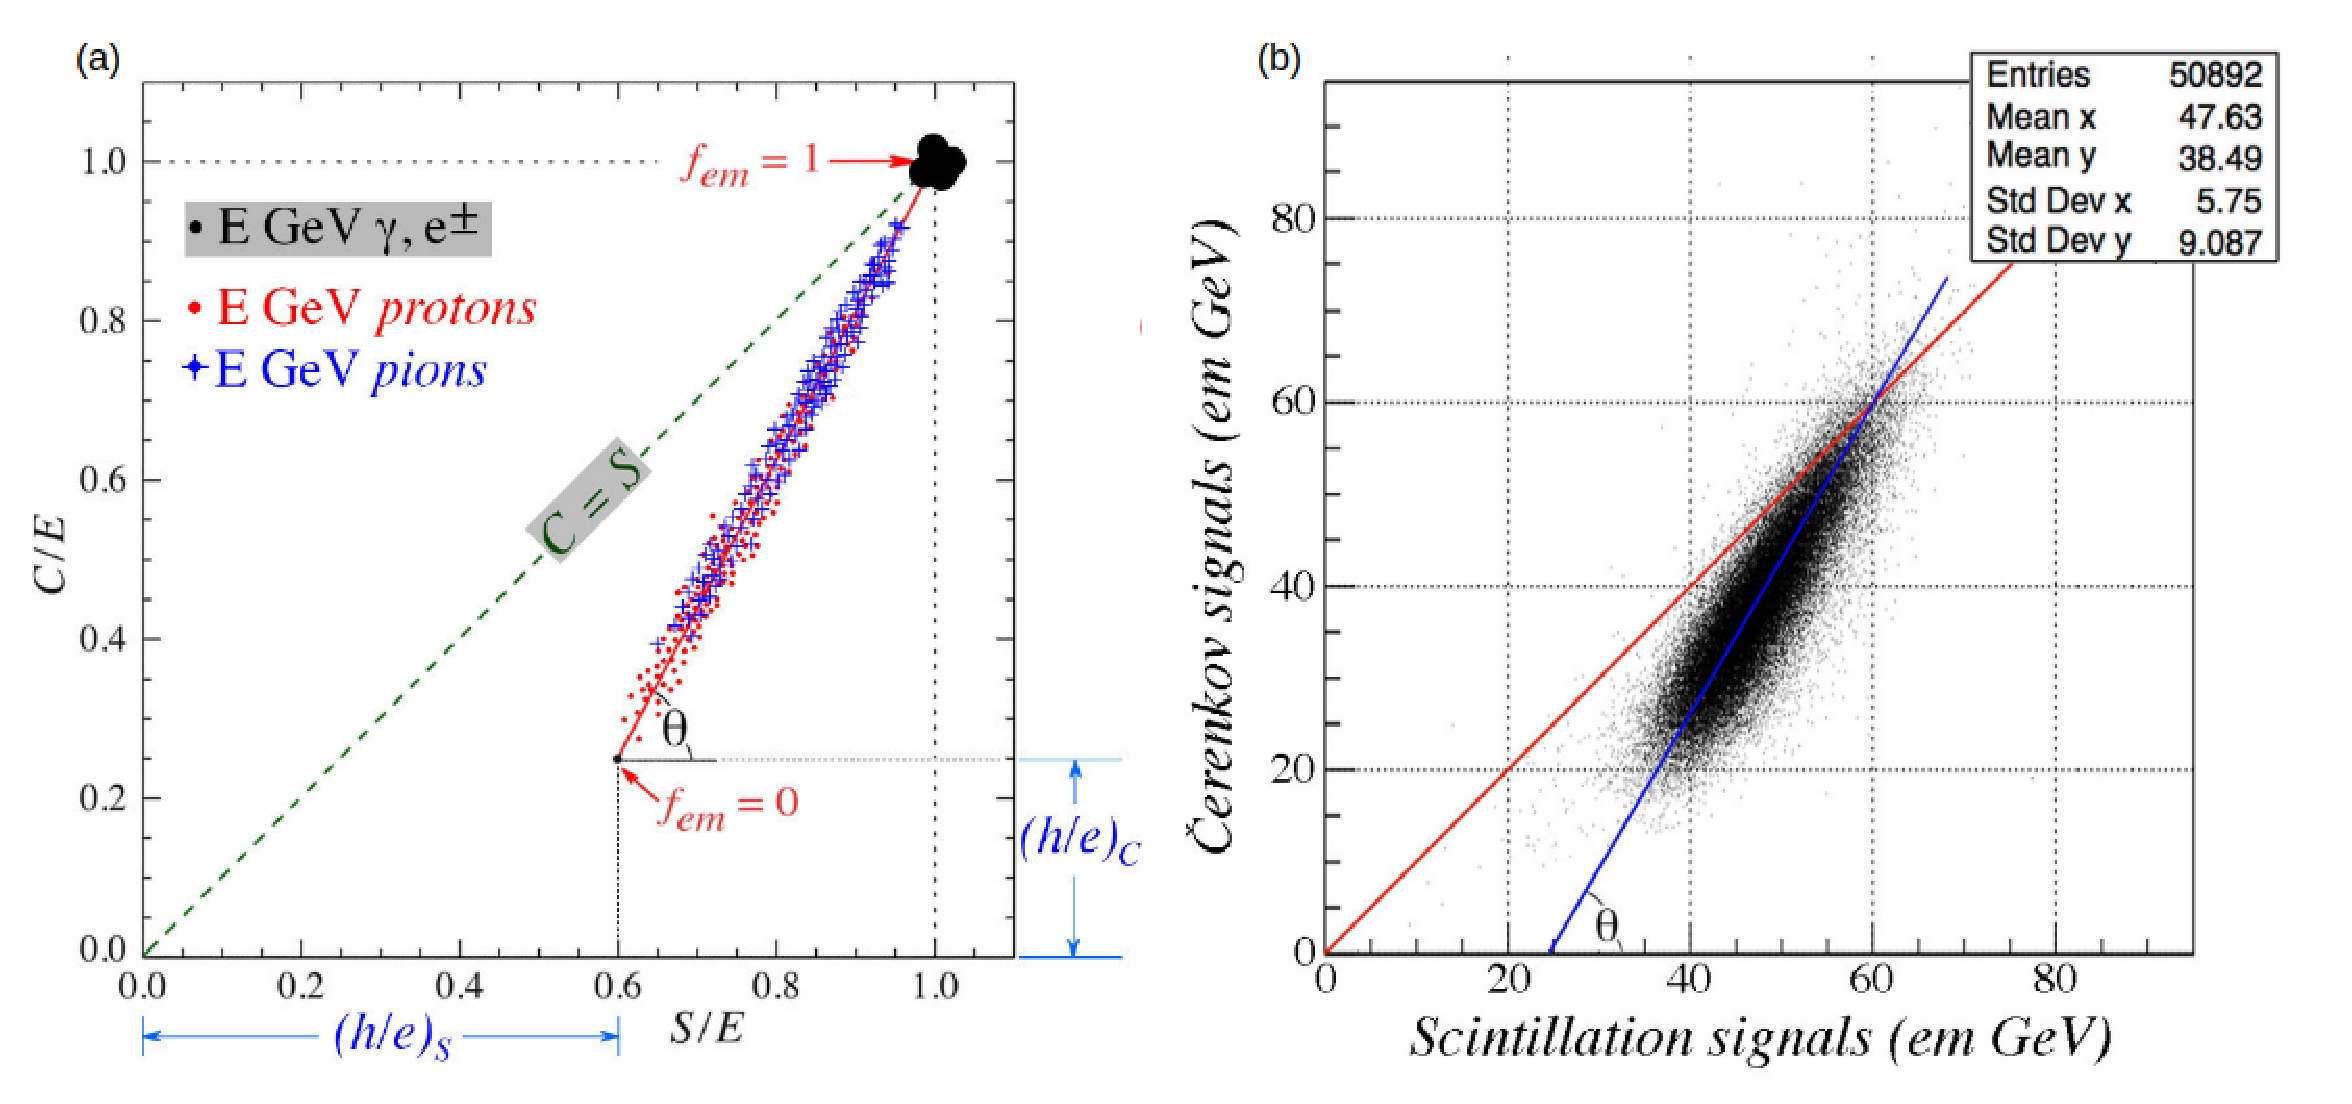
\includegraphics[width=\columnwidth]{Figures/Calorimetry/theta_angle5.eps}
    %%% 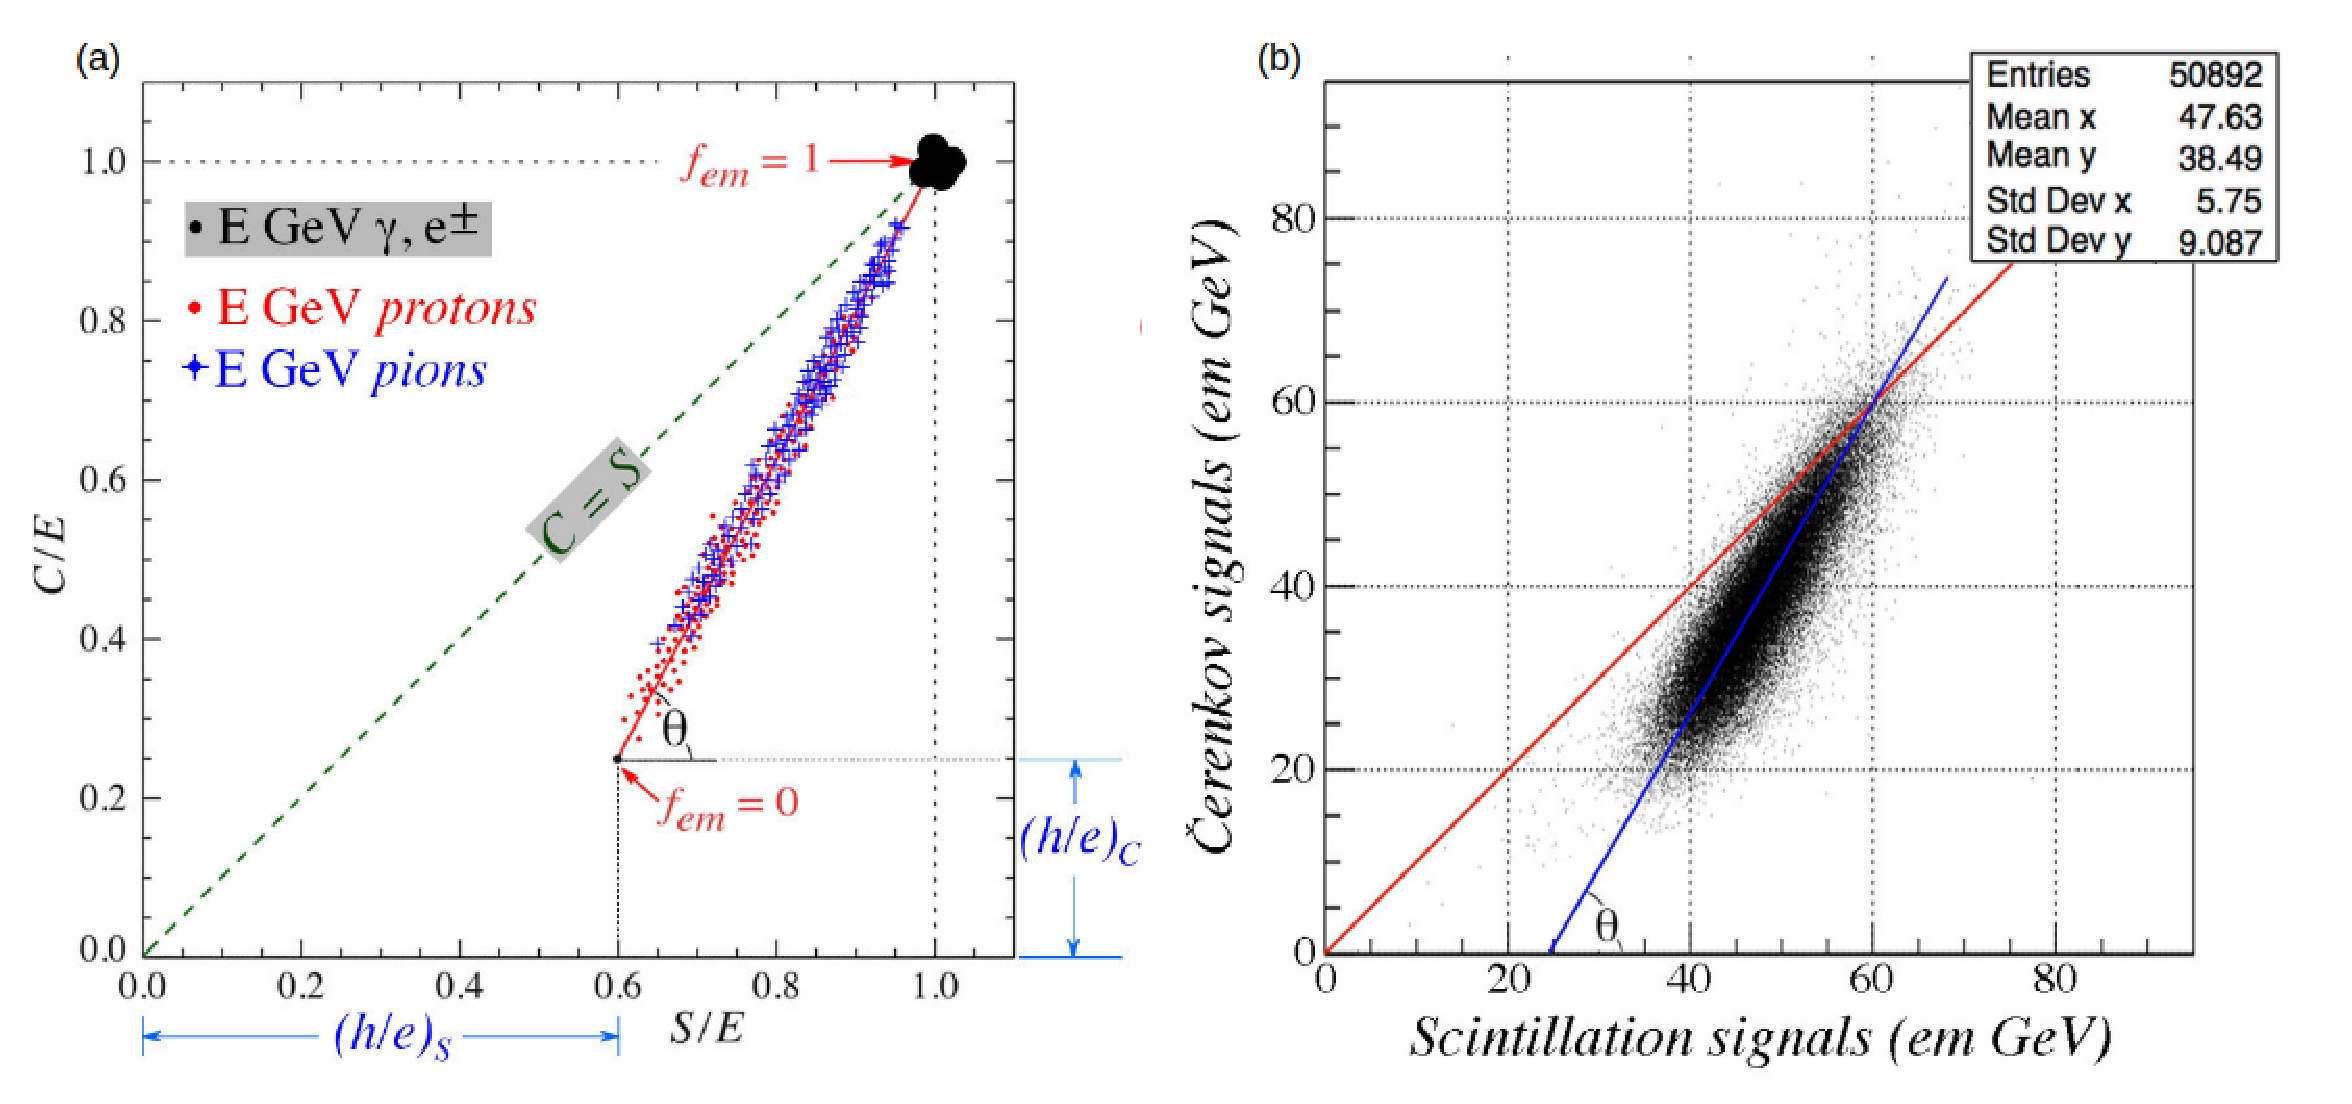
\includegraphics[width= 0.55\textwidth]{Figures/Calorimetry/theta_angle5.eps}
  \caption{(a) Scatter plot of C/E versus S/E in a dual-readout
calorimeter for $p$ and $\pi$; (b) scatter plot of C versus S signals for
60 GeV pions in the RD52 dual-readout lead/fibre calorimeter.}
  \label{fig:theta_angle5}
\end{figure}

The plot in Figure~\ref{fig:theta_angle5}(b) shows the data points located
on a locus, clustered around a line that intersects the C/S = 1 line at
the beam energy of 60 GeV. $\chi$ is the energy-independent slope of the
event locus. This is to be expected. In first approximation, the signal
generated in the \v{C}erenkov fibers is produced only by the $em$
components of the hadron showers. The larger the $em$ fraction $f_{em}$,
the larger the C/S signal ratio. Events in which (almost) the entire
hadronic energy is deposited in the form of $em$ shower components give
signals very similar to those from 60 GeV electrons and are, therefore,
represented by data points located near (S=60, C=60) in the plot.

All signals are relative to the $em$ scale meaning that both the
\v{C}erenkov and the scintillation responses have to be calibrated with
electrons only, i.e. no hadronic calibration is required. This is one of
the most qualifying point of dual-readout calorimetry.

The effectiveness of this approach has been probed by the DREAM/RD52
collaboration over a 15-year research program with a variety of detector
solutions. Results and
simulations~\cite{rd52_pid2014,rd52_em2014,rd52_sim2014,rd52_em2016,wigmans_nimA824,rd52_hadr2017}
provide, so far, confidence
that a fibre-sampling calorimeter, even without longitudinal segmentation,
may meet the requirements of the CepC physics programme in a
cost-effective way. Linearity and energy resolution, for both $em$ and
hadronic showers, $e/\pi/\mu$ separation, spatial resolution, all show
adequate performance.

\subsection{Layout and Mechanics}

\subsubsection{Layout}

A possible projective layout has been studied by the 4th Detector
Collaboration and described in its LoI~\cite{4th_loi}.
Assuming the converter to be
copper, the calorimeter is a copper matrix loaded with 1 mm diameter, 1 mm
apart, alternate scintillating and clear (for \v{C}erenkov light
detection) fibres. About 200 $cm$ (10 $\lambda$) long, projective towers
cover (at $\theta \sim 90^\circ$) about 1.4$^{\circ}$ in both $\phi$ and
$\theta$, with of the order of 2000 fibres per tower. The dimensions of
the inner faces in the barrel section depend on $\theta$, and increase
going in the forward direction. The sampling fraction is kept constant by
fibres starting at different depths inside each tower.

This layout has been already imported in the simulations for the CepC
detector and will be validated in the next months.

\subsubsection{Mechanics (Material Choice and Machining)}

Both lead and copper have been used as absorber materials by the
DREAM/RD52 collaboration. Their main properties are:

\begin{align}
Lead: \rho= 11.3\ g/cm^3,\ X_0= 0.56\ cm,\ \rho_{Mol}= 1.60\ cm,\ \lambda_{int}= 170\ mm
\end{align}
\begin{align}
Copper: \rho= 8.96\ g/cm^3,\ X_0= 1.44\ cm,\ \rho_{Mol}= 1.56\ cm,\ \lambda_{int}= 151\ mm
\end{align}

meaning that, for hadronic showers, a full-coverage solution with lead
will give broader and longer showers and a total mass 42\% heavier than
using copper. A full-containment $ 3 \times 3 \times 10\ \lambda^3 $
prototype will need about 5 tons of material with lead and 2.8 tons with
copper.

An even stronger reason in favour of copper is the fact that, being the
\v{C}erenkov light almost exclusively produced by the $em$ shower
components and the (e/mip) ratio 50\% higher for copper than for lead, the
\v{C}erenkov light yield should be significantly higher in copper,
resulting in a better hadronic resolution.

On the other hand, copper extrusion, with the required tolerances in
planarity and groove parallelism, is not yet an established industrial
process. A variety of techniques (extrusion, rolling, scraping and
milling) for machining the converter layers have been tested, essentially
by John Hauptman and collaborators at Iowa State University and by
Fabrizio Scuri at INFN-Pisa. None has been qualified for a large-scale
production and identifying an industrial and cost-effective process,
including moulding, is a relevant issue.

In the 3-year R\&D INFN program, under discussion, the identification of
an industrial procedure to produce the converter layers is one key point.

Alternative copper alloys (brass, bronze) will be investigated as well,
both for addressing the production process issues and for optimising the
detector performance.

\subsection{DREAM/RD52 Prototype Studies}

Different prototypes were built and studied by the DREAM/RD52
collaboration, with copper or lead as absorber. A summary of the most
significant results~\cite{rd52_pid2014,rd52_em2014,rd52_sim2014,rd52_em2016,wigmans_nimA824,rd52_hadr2017} is given, in particular for the matrices
built in 2012: a matrix of 9 lead modules and a matrix of 2 copper
modules, each module $9.3 \times 9.3 \times 250\ cm^3$ (see
Figure~\ref{fig:AllDet} for the mechanical details, the first DREAM
calorimeter built in 2003 is also shown on the top). From the readout
point of view, the calorimeter was arranged as in
Figure~\ref{fig:rd52_2012}.

\begin{figure}
  \centering
   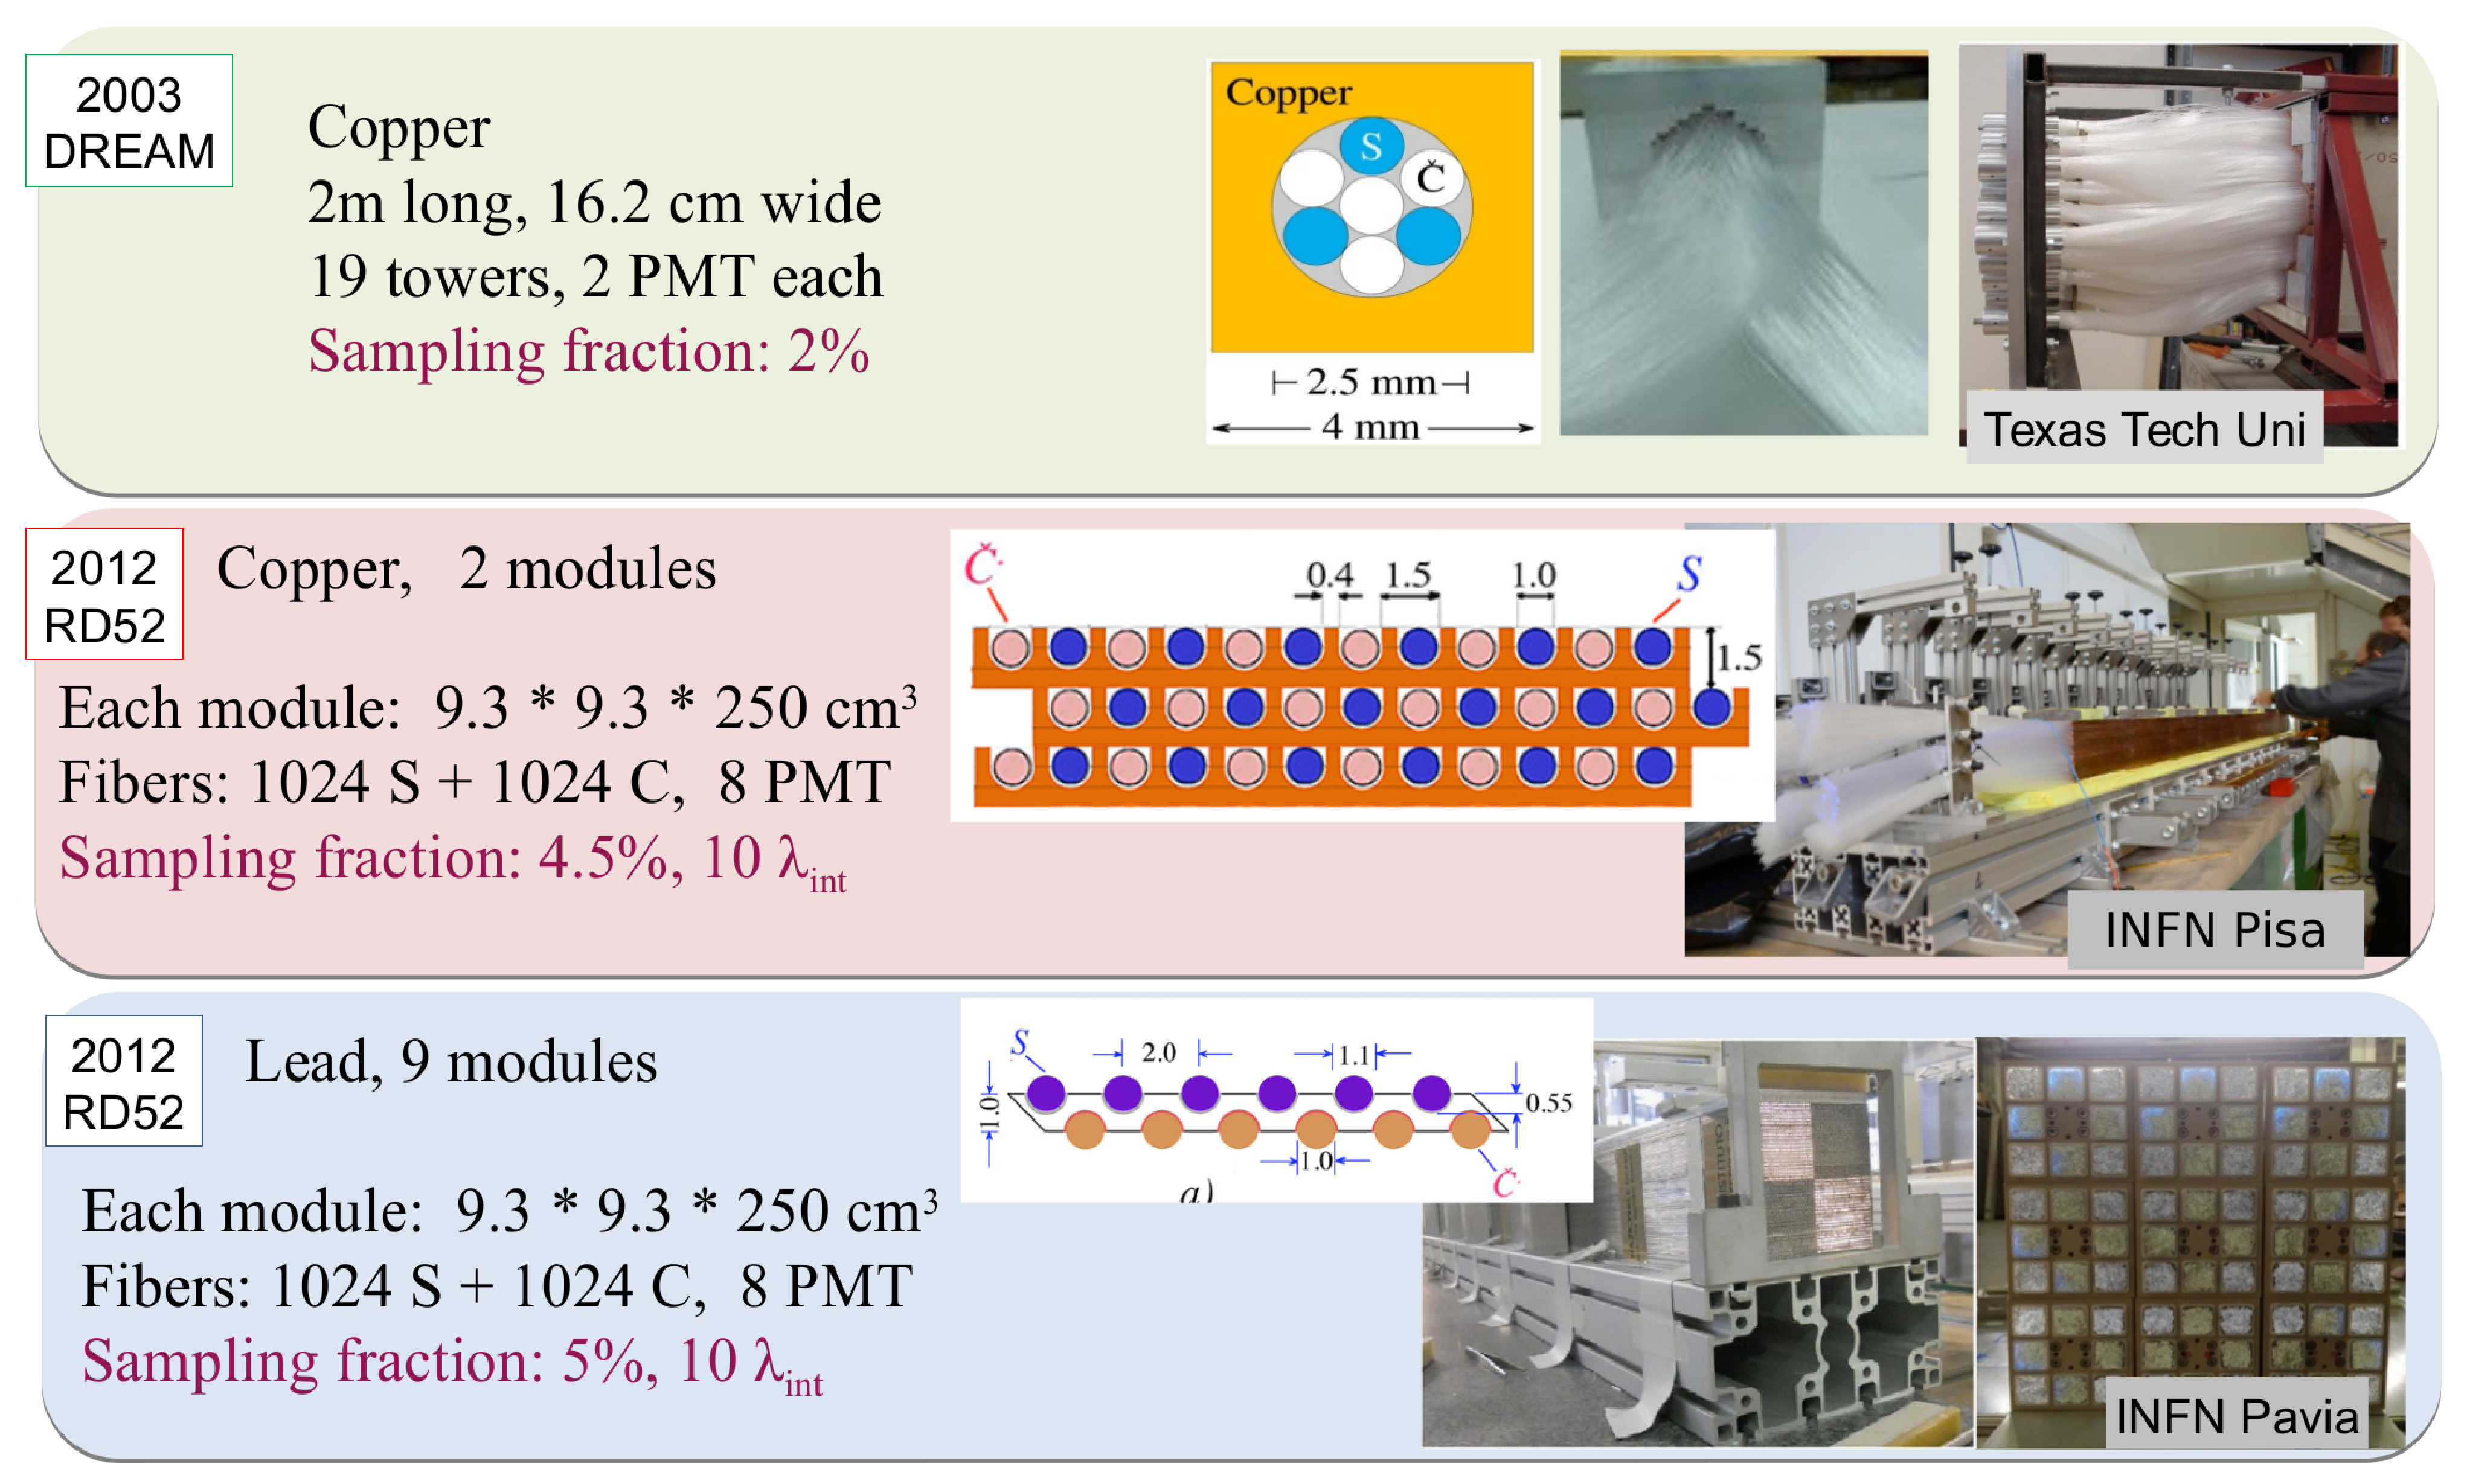
\includegraphics[width=\columnwidth]{Figures/Calorimetry/AllDet.eps}
    %%% 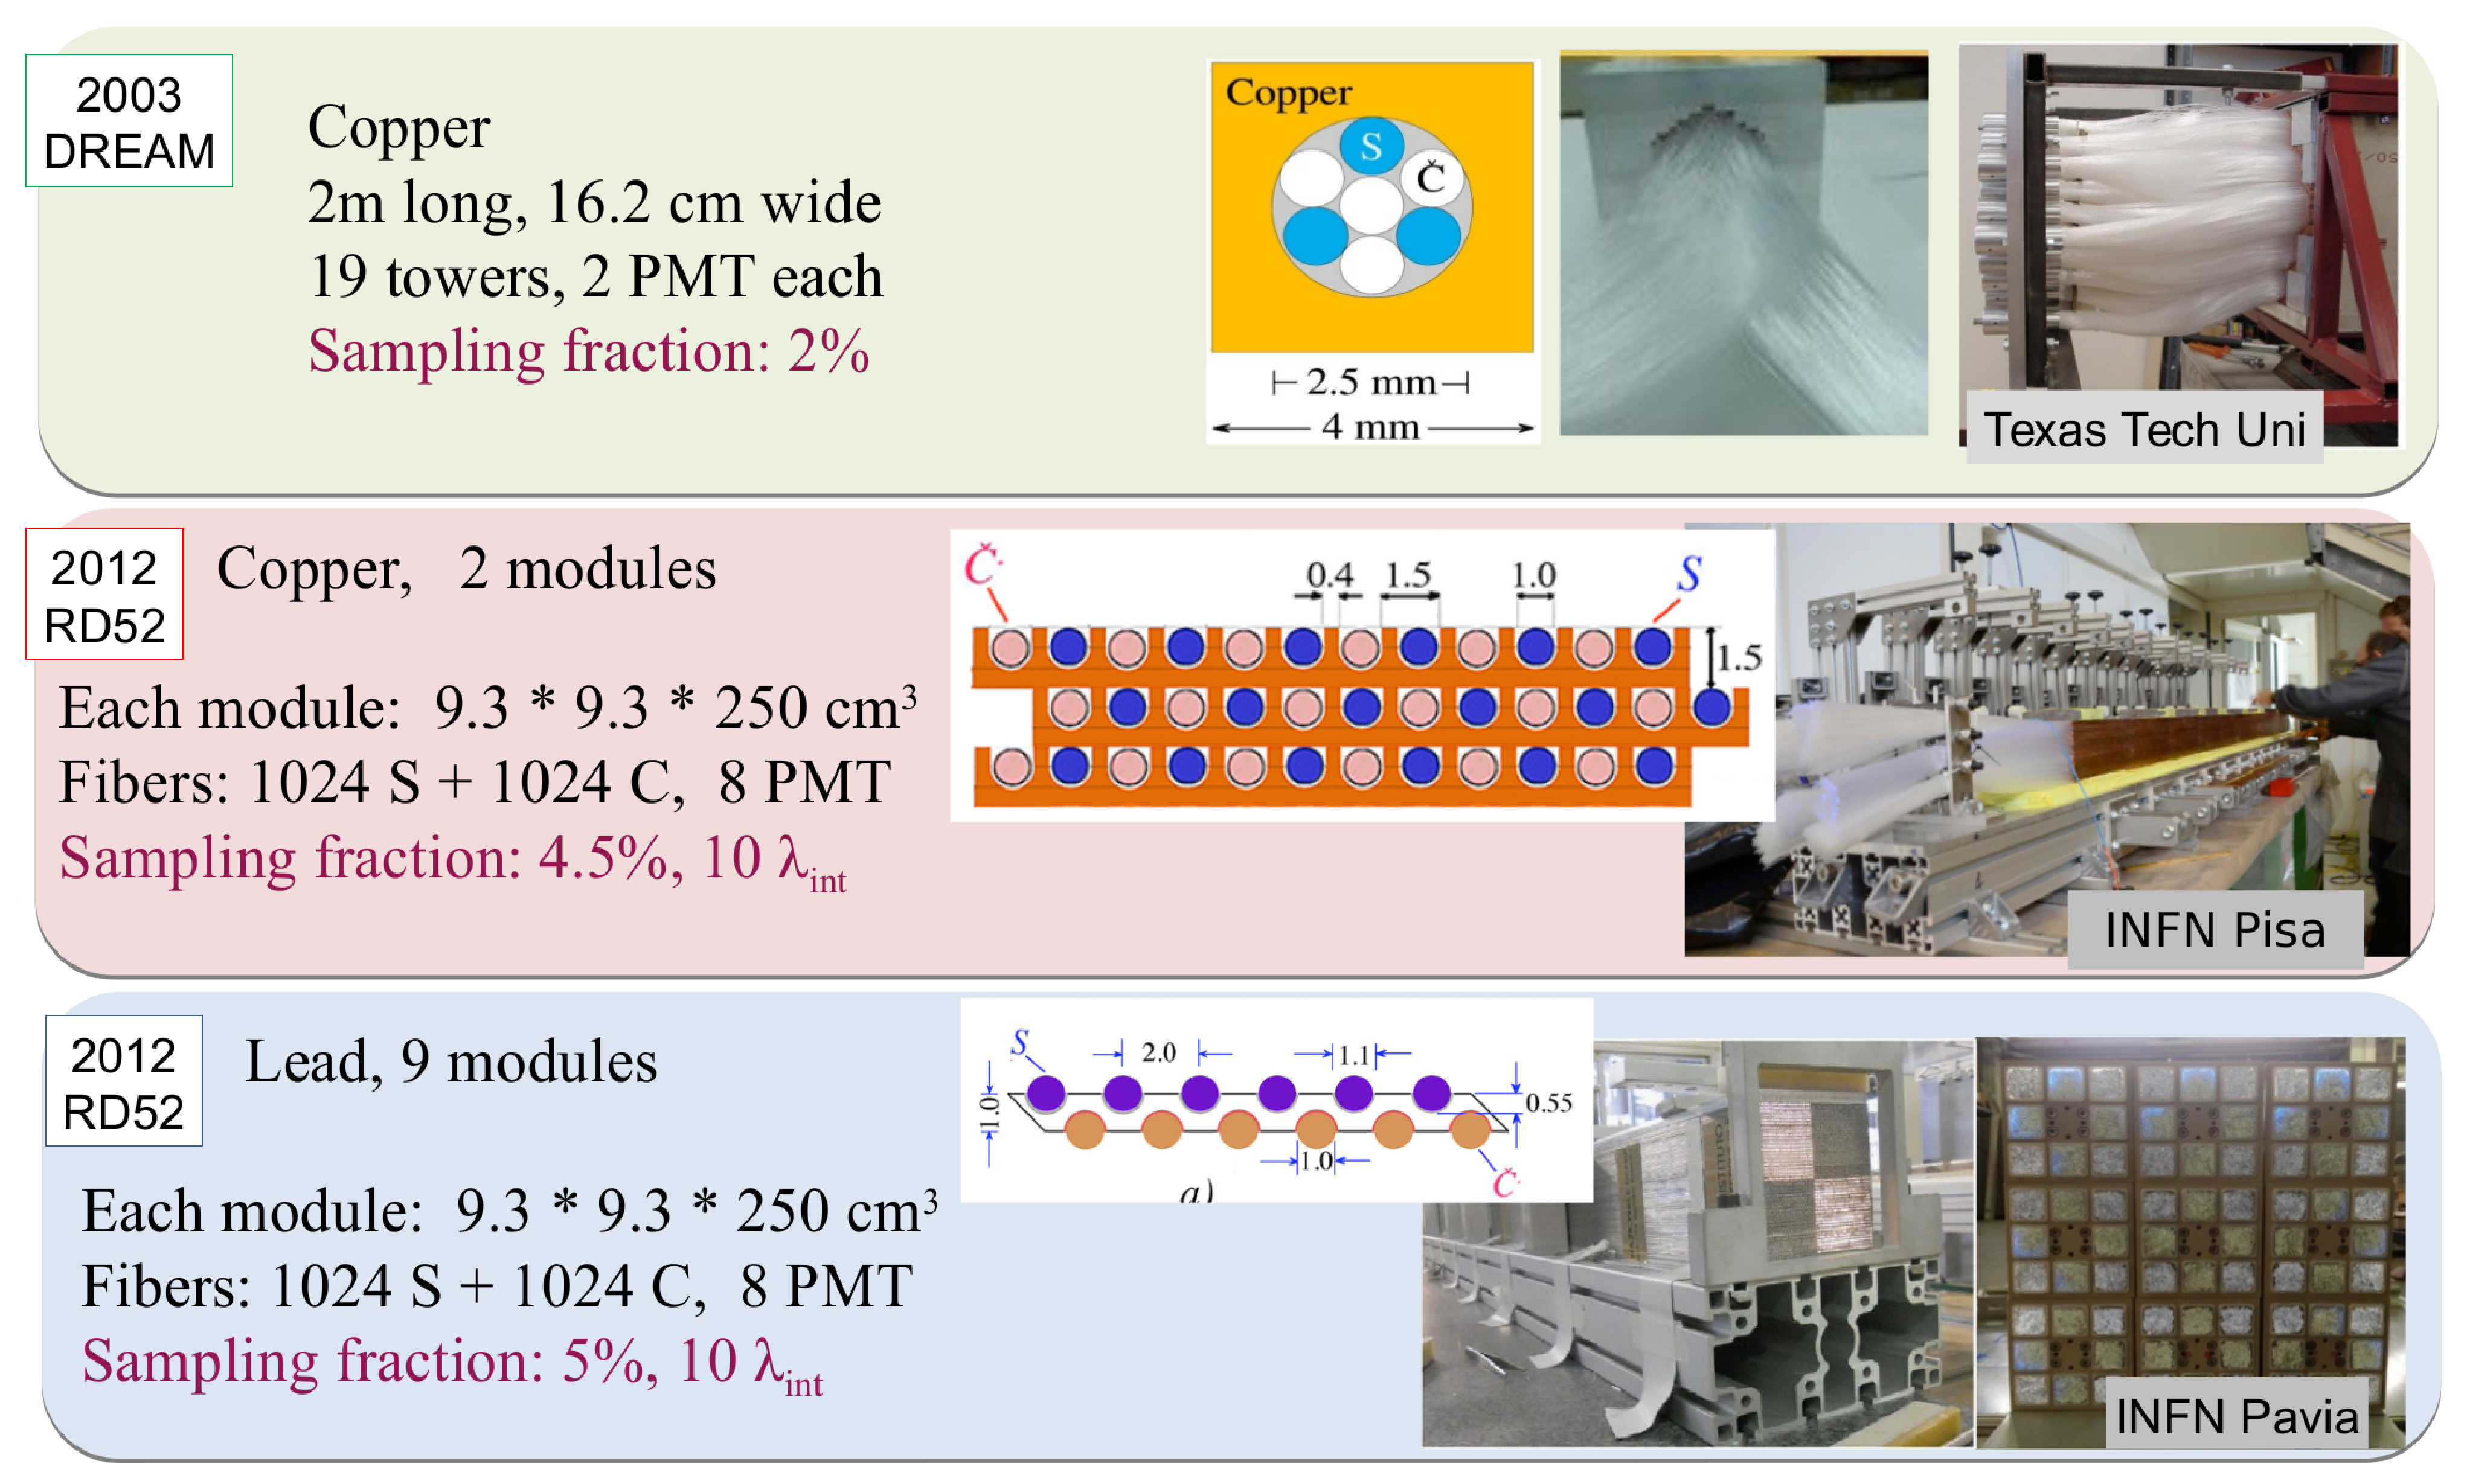
\includegraphics[width= 0.55\textwidth]{Figures/Calorimetry/AllDet.eps}
  \caption{The DREAM calorimeter (top), built in 2003, and the RD52
prototypes, with copper (middle) and lead (bottom), built in 2012.}
  \label{fig:AllDet}
\end{figure}

\begin{figure}
  \centering
   %%% 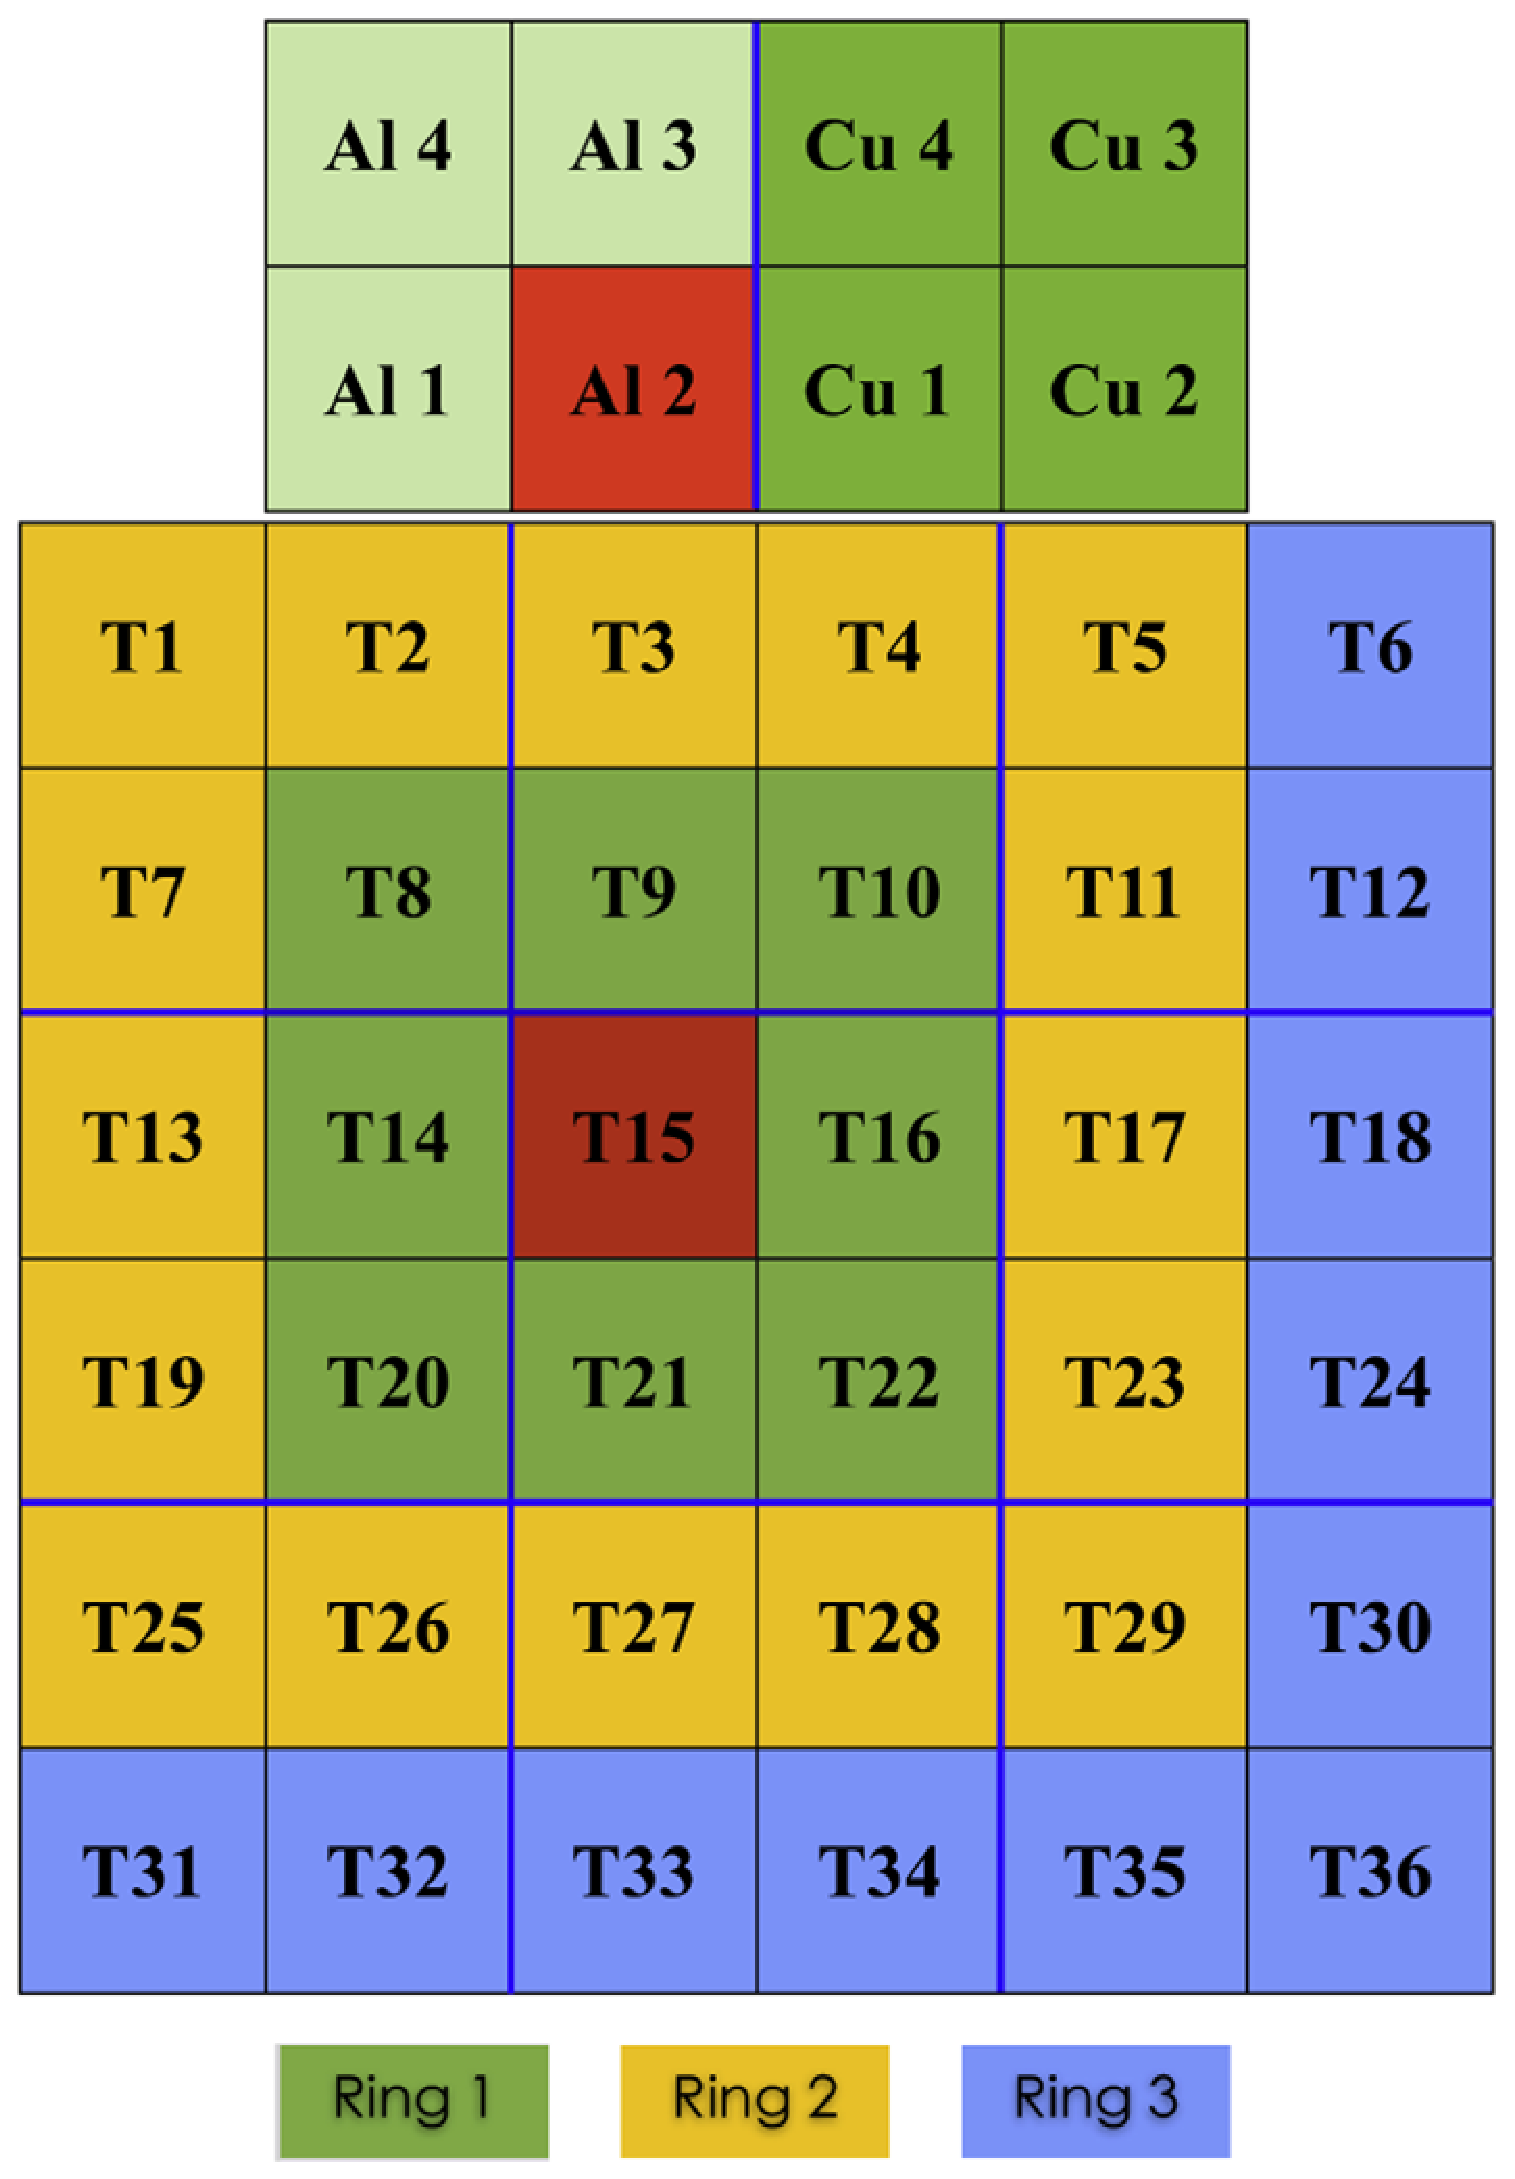
\includegraphics[width=\columnwidth]{Figures/Calorimetry/rd52_2012.eps}
   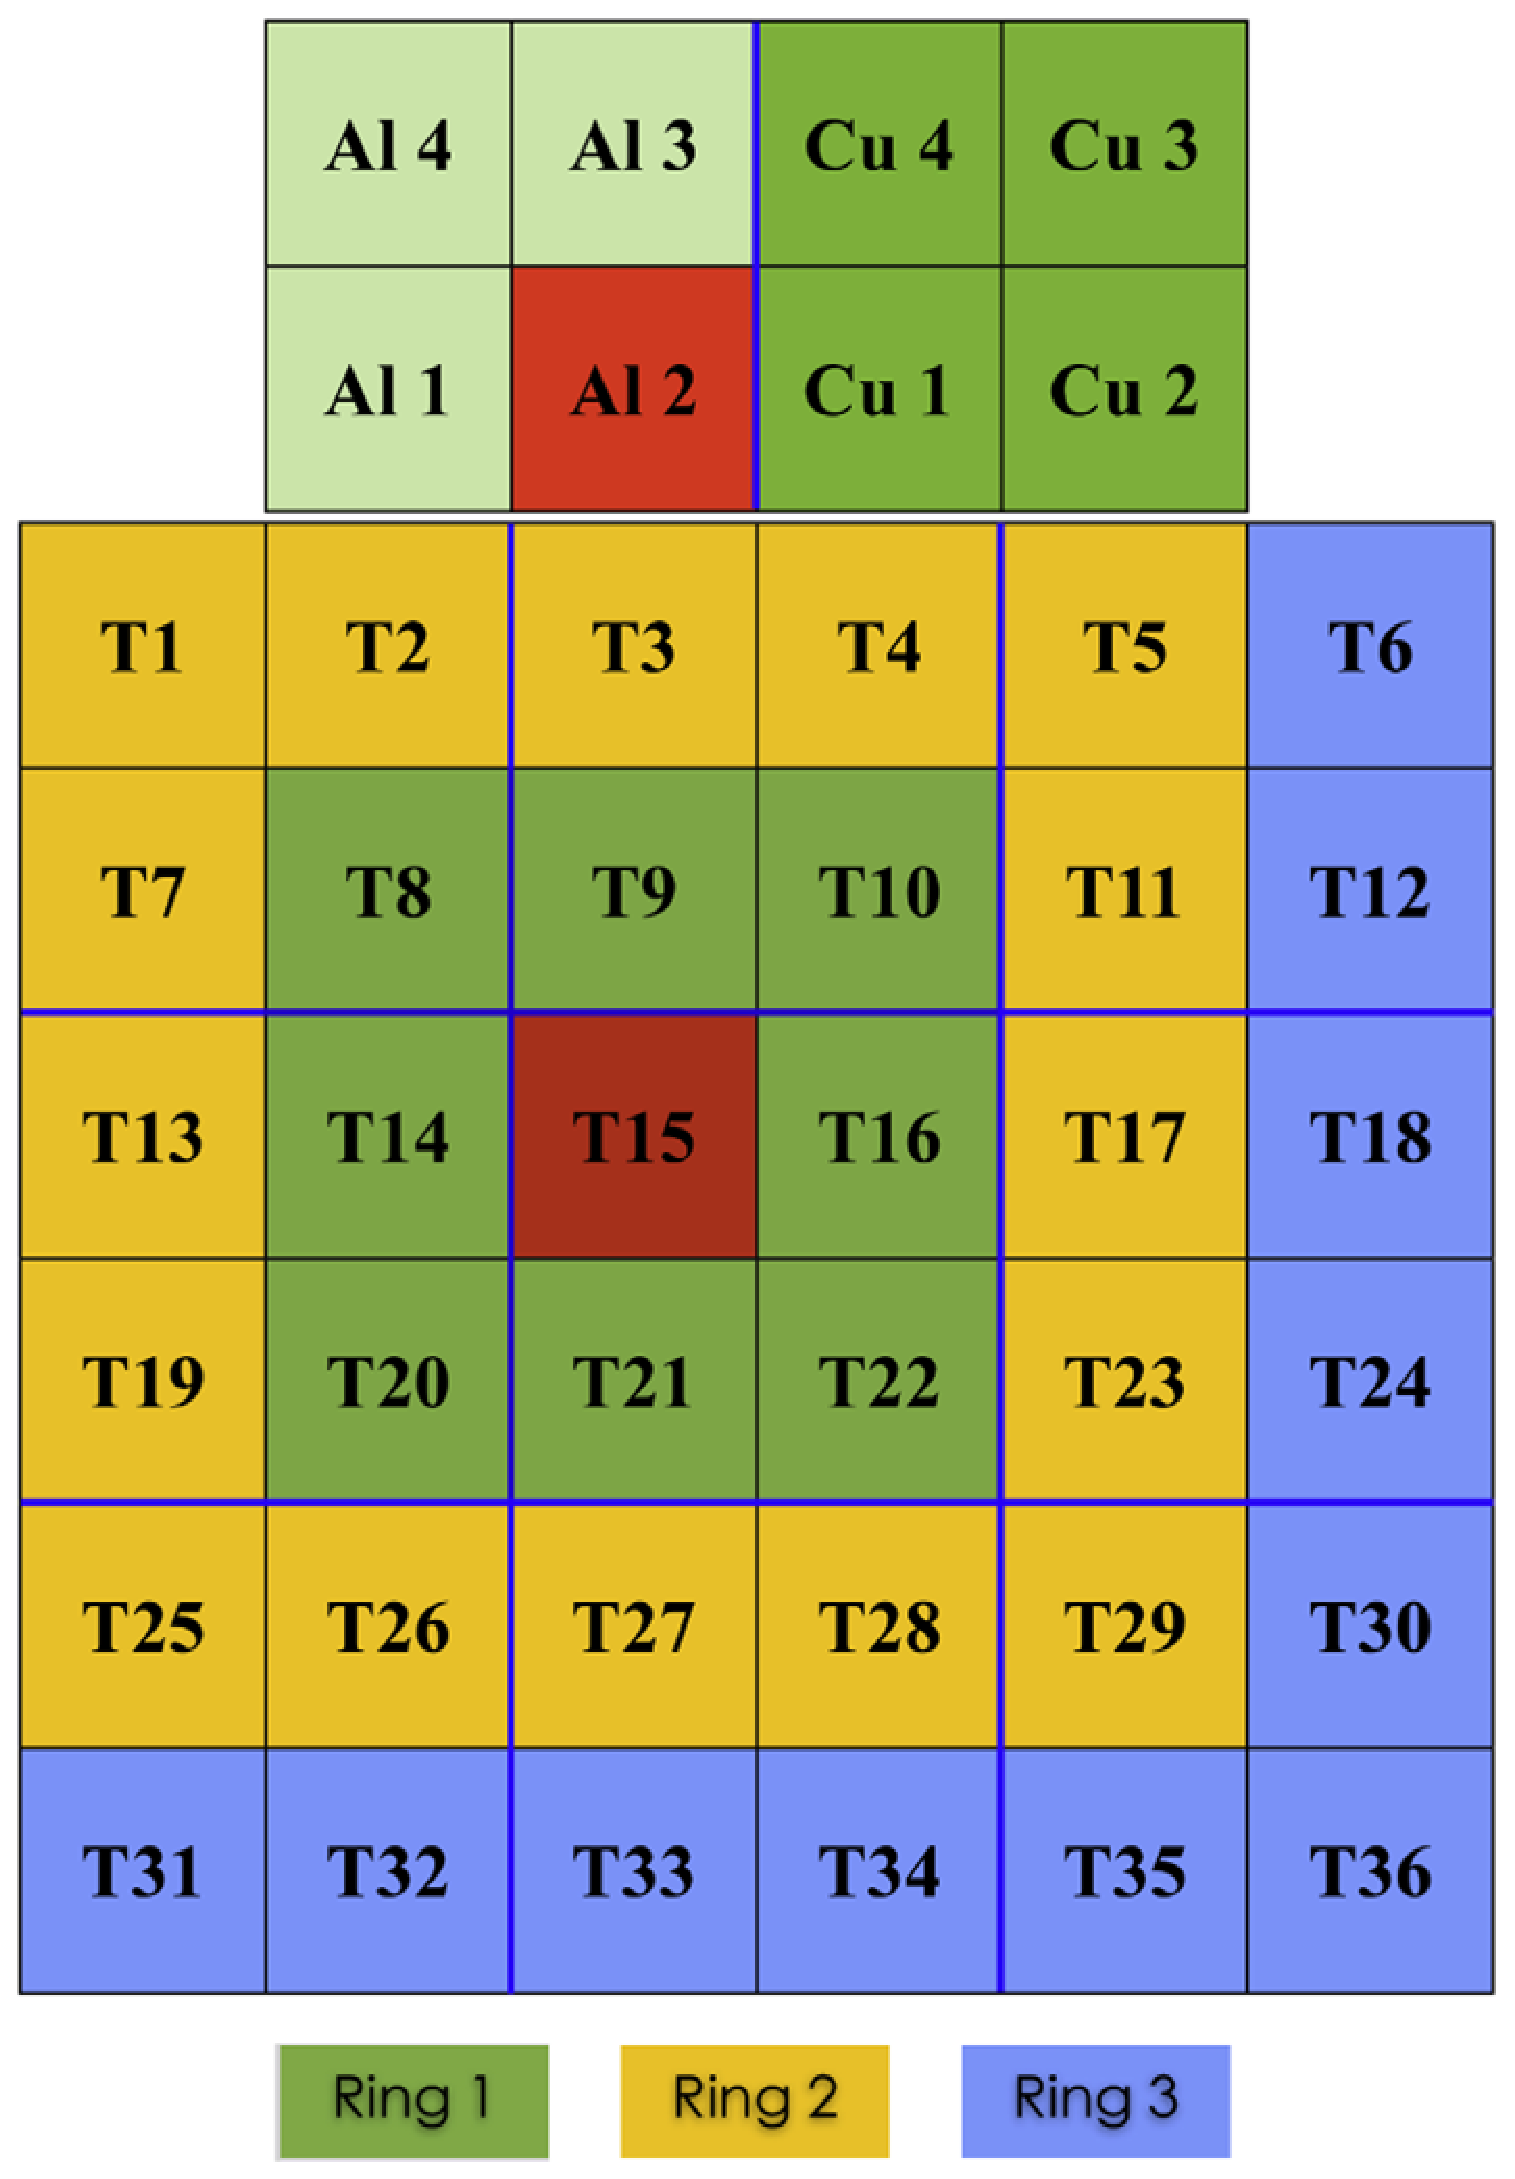
\includegraphics[width= 0.55\textwidth]{Figures/Calorimetry/rd52_2012.eps}
  \caption{The RD52 calorimeter as tested at the end of 2012. It consisted
of 9 lead-based modules, each consisting of 4 towers (towers 1-36), and 2
copper-based modules, placed on top of the lead array. Each tower was
readout by two photomultipliers, one for scintillation and one for
\v{C}erenkov light detection. The left copper module (of which the towers
are marked as “Al”) was equipped with \v{C}erenkov fibres with an
aluminised upstream end face. For the measurements described in this
paper, the particle beams were typically steered in the center of tower
T15.}
  \label{fig:rd52_2012}
\end{figure}

\subsubsection{Electromagnetic Performance}

In Figure~\ref{fig:emLin} the linearity of the response for both matrices
is shown. The range of measurement is different for the two (spanning 6-60
GeV for Cu and 60-150 GeV for Pb). The deviations for the very first
points ($\lesssim 10\ GeV$) are likely due to the spread of the energy of
the beam particles.

\begin{figure}
  \centering
   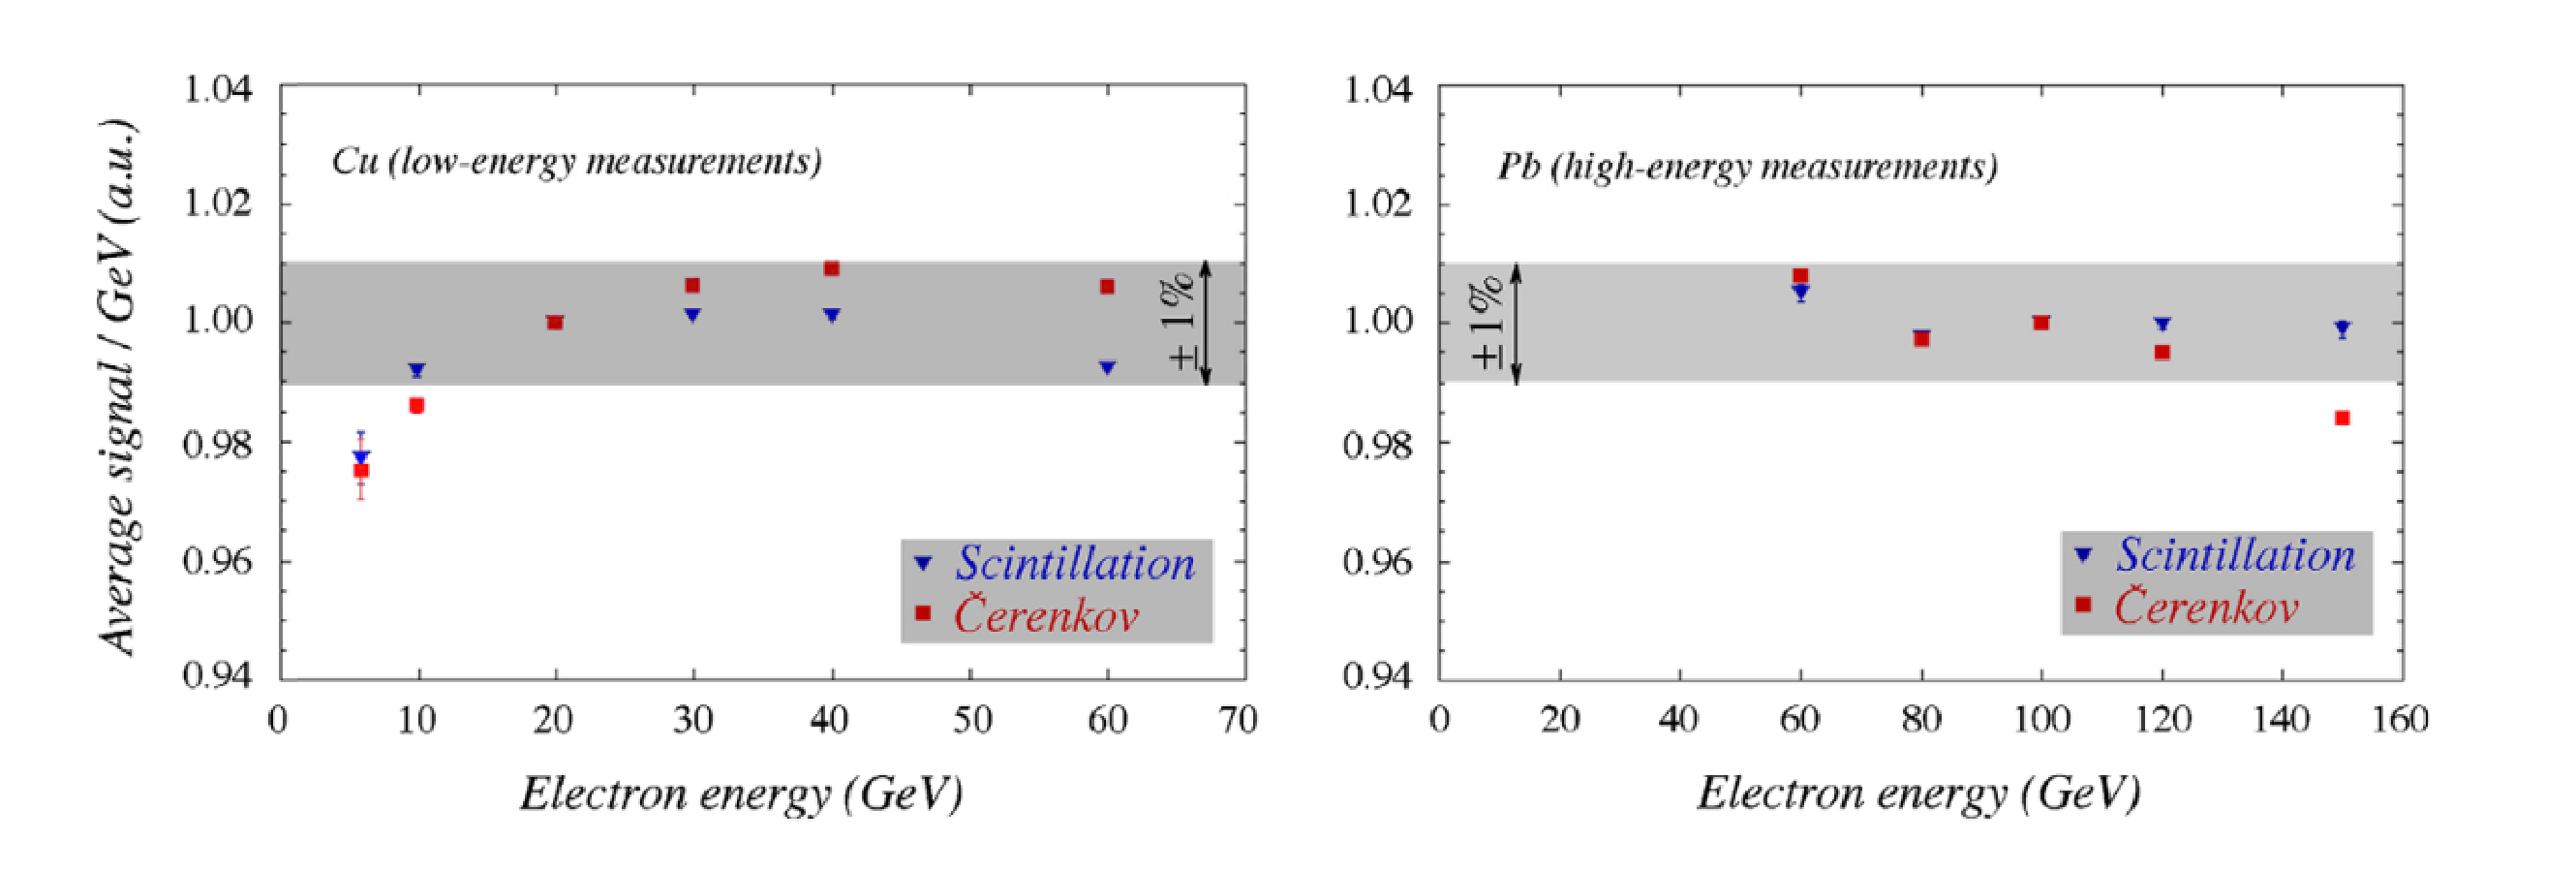
\includegraphics[width=\columnwidth]{Figures/Calorimetry/emLin.eps}
    %%% 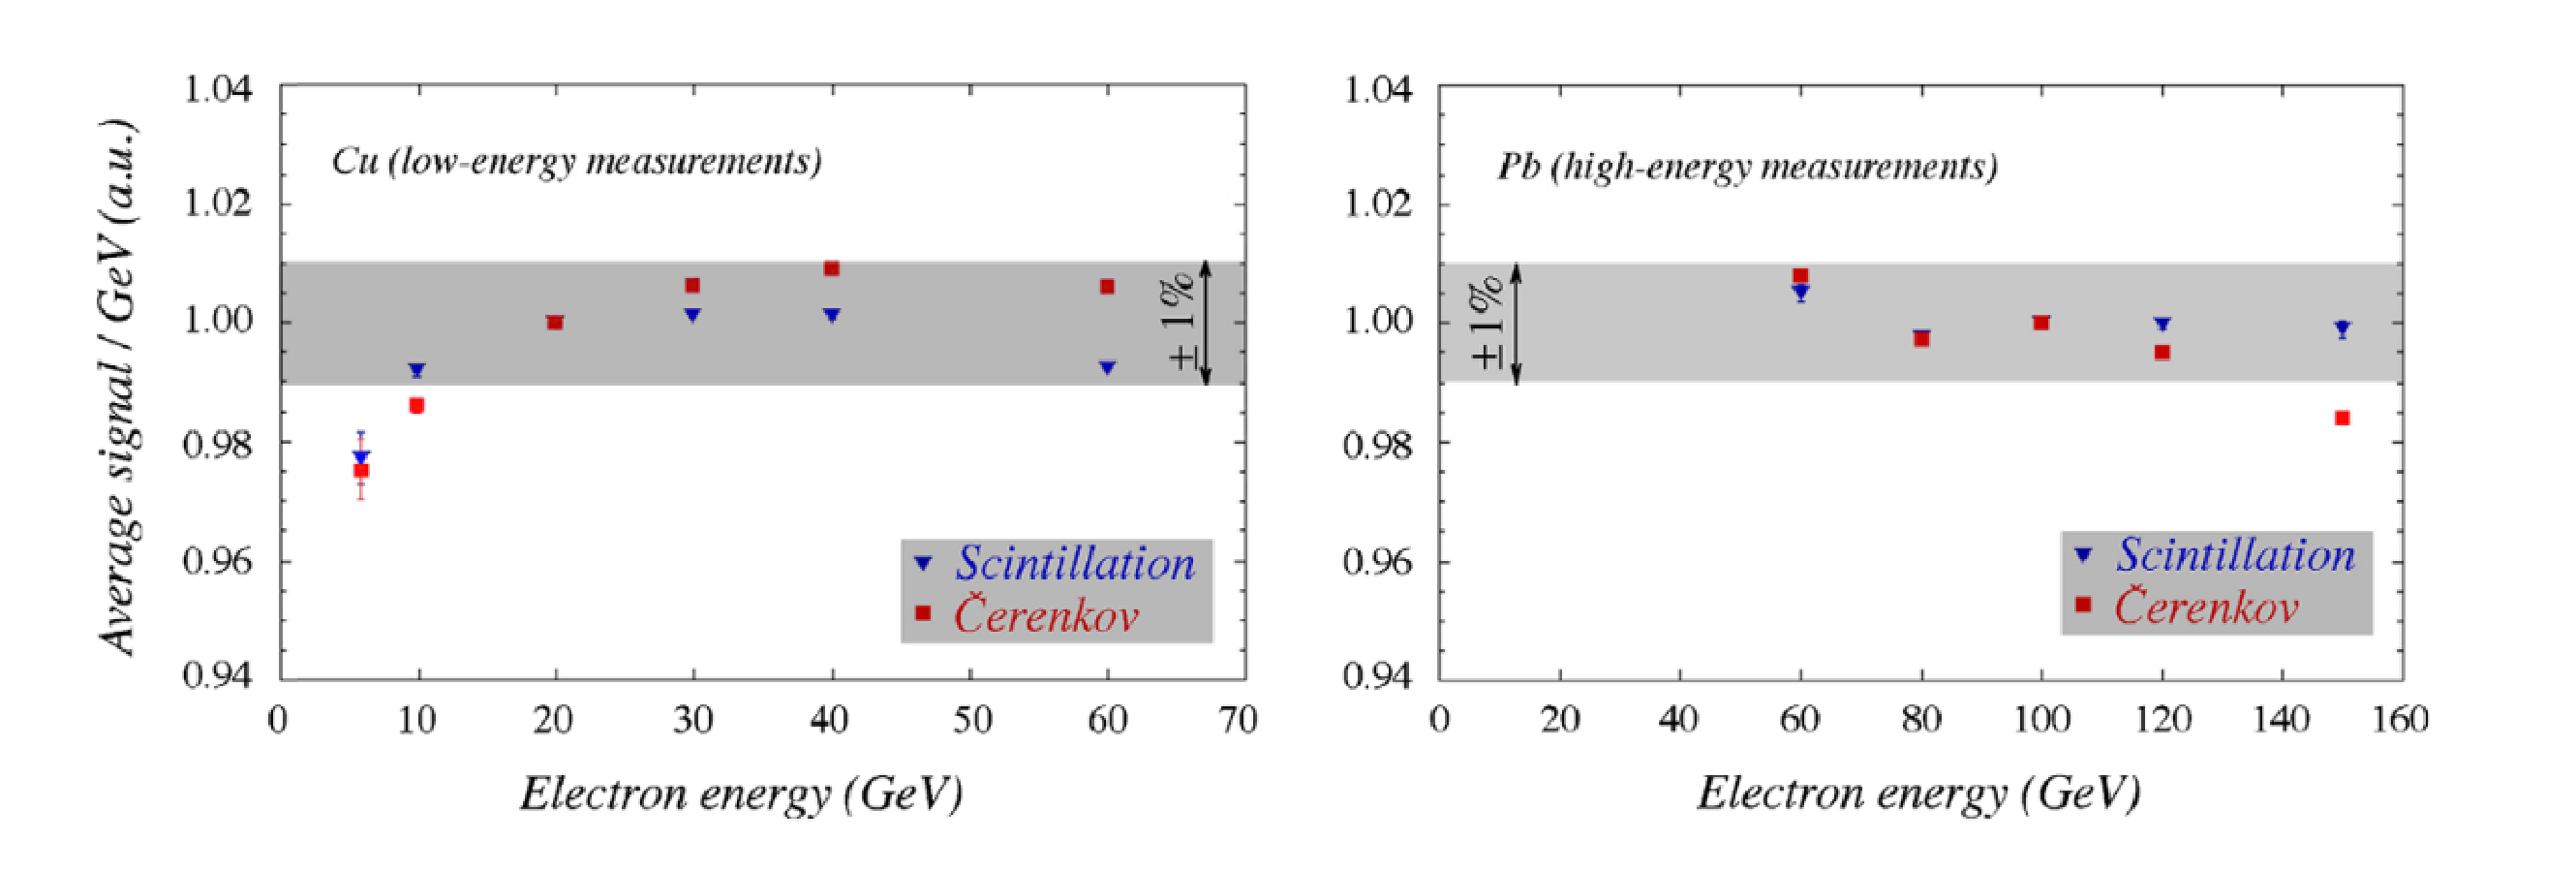
\includegraphics[width= 0.55\textwidth]{Figures/Calorimetry/emLin.eps}
  \caption{The linearity of the copper (left) and lead (right) based fibre
calorimeters for em shower detection in the scintillation and \v{C}erenkov
channels.}
  \label{fig:emLin}
\end{figure}

Figure~\ref{fig:emProf} shows the radial shower profile and the sensivity
to the impact point: the core of the signal spans just few mm.
Figure~\ref{fig:impactScan} shows the dependence of the S signal on the
impact point for particles entering parallel to the fibres. This
introduces a constant term in the resolution that can be avoided with a
small tilt of the fibre axis. In the C fibres, the problem doesn't show up
since the early (collimated) part of the shower produces photons outside
the numerical fibre aperture.

\begin{figure}
  \centering
   \includegraphics[width=\columnwidth]{Figures/Calorimetry/emProf.eps}
    %%% \includegraphics[width= 0.55\textwidth]{Figures/Calorimetry/emProf.eps}
  \caption{The signal from a 1 mm wide beam of 100 GeV electrons, as a
function of the impact point (a), and the lateral shower profiles derived
from this measurement (b).}
  \label{fig:emProf}
\end{figure}

\begin{figure}
  \centering
   %%% \includegraphics[width=\columnwidth]{Figures/Calorimetry/impactScan.eps}
   \includegraphics[width= 0.55\textwidth]{Figures/Calorimetry/impactScan.eps}
  \caption{The scintillation signal for 100 GeV electrons developing
showers in the lead matrix as a function of the beam impact point.}
  \label{fig:impactScan}
\end{figure}

For the reconstruction of the energy of $em$ showers, C and S signals
provide independent uncorrelated measurements, with different sensitivity
of the response. They are affected by different problems: S signals have a
photo-electron statistics of at least one order of magnitude higher than C
signals, and their fluctuations are largely dominated by the sampling
fluctuation of the energy deposits. C signal fluctuations are generally
dominated by the limited photo-electron statistics, expecially at low
energies. Nevertheless, for C signals, the constant term is negligible
giving a better resolution at high energies. Averaging the two measures
improves the resolution up to a factor of $\sqrt 2$. Separate and combined
(unweighted) results for the copper matrix are shown in
Figure~\ref{fig:40gevRes} for 40 GeV electrons.

\begin{figure}
  \centering
   \includegraphics[width=\columnwidth]{Figures/Calorimetry/40gevRes.eps}
   %%% \includegraphics[width= 0.55\textwidth]{Figures/Calorimetry/40gevRes.eps}
  \caption{Signal distributions for 40 GeV electrons in the copper-fibre
calorimeter: from the sum of the scintillating fibres (a), of the
\v{C}erenkov fibres (b), of all fibers (c). The angle of incidence of the
beam particles ($\theta,\ \phi$) was ($1.5^\circ, 1.0^\circ$). The size of
the beam spot was $10 \times 10\ mm^2$.}
  \label{fig:40gevRes}
\end{figure}

In Figure~\ref{fig:CuPbRes}, the electromagnetic resolution is shown for
the 2 matrices.

\begin{figure}
  \centering
   \includegraphics[width=\columnwidth]{Figures/Calorimetry/CuPbRes.eps}
   %%% \includegraphics[width= 0.55\textwidth]{Figures/Calorimetry/CuPbRes.eps}
  \caption{The energy resolution for electrons in the copper-fibre module
(left) and in the lead-fibre module (right), as a function of the beam
energy. Shown are the results for the two types of fibres, and for the
combined signals. The angle of incidence of the beam particles ($\theta,\
\phi$) was ($1.5^\circ, 1.0^\circ$). The size of the beam spot was $10
\times 10\ mm^2$.}
  \label{fig:CuPbRes}
\end{figure}

\subsubsection{Hadronic Performance}

The RD52 lead matrix response was studied with pion and proton beams~\cite{rd52_hadr2017}.  High-multiplicity events ("jets") were also generated by means of
a target. The energy was reconstructed with the dual-readout relation (Eq.
4), that restores a gaussian behaviour and linearity of the response
(Figure~\ref{fig:DRsignal} and Figure~\ref{fig:linResp}).

\begin{figure}
  \centering
   \includegraphics[width=\columnwidth]{Figures/Calorimetry/DRsignal.eps}
   %%% \includegraphics[width= 0.55\textwidth]{Figures/Calorimetry/DRsignal.eps}
  \caption{Signal distributions for 20 GeV $\pi^-$ particles. Shown are
the measured \v{C}erenkov (a) and scintillation (b) signal distributions
as well as the signal distribution obtained by combining the two signals
according to Equation 4, with $\chi = 0.45$ (c).}
  \label{fig:DRsignal}
\end{figure}

\begin{figure}
  \centering
   %%% \includegraphics[width=\columnwidth]{Figures/Calorimetry/linResp.eps}
   \includegraphics[width= 0.55\textwidth]{Figures/Calorimetry/linResp.eps}
  \caption{The hadronic response for single pions. Shown are the average
\v{C}erenkov signal and the dual-readout signal (Eq. 4) per unit deposited
energy, as a function of the pion energy.}
  \label{fig:linResp}
\end{figure}

The comparison of $p$ and $\pi$ signals at 80 GeV is shown in
Figure~\ref{fig:pi_prot}, confirming that the method largely compensates
for the differences in shower composition.

\begin{figure}
  \centering
   %%% \includegraphics[width=\columnwidth]{Figures/Calorimetry/pi_prot.eps}
   \includegraphics[width= 0.77\textwidth]{Figures/Calorimetry/pi_prot.eps}
  \caption{Signal distributions for the \v{C}erenkov signals from 80 GeV
$\pi^+$ (a) and protons (b), as well as the dual-readout total signals for
80 GeV $\pi^+$ (c) and protons (d).}
  \label{fig:pi_prot}
\end{figure}

The limited lateral size of the matrix (about 1 $\lambda$) allows to
collect, in average, $\sim 90\%$ of the shower energy so that leakage
fluctuations dominate the resolution capability. Leakage counters were
used to select events about fully contained (that of course, tend to have
a higher $f_{em}$). The resolution improves by a factor of almost 2 in
this case (Figure~\ref{fig:leak_eff}). A second effect affecting
resolution is the light attenuation in the fibres, that causes early
starting showers to be observed at lower signal values. The hadronic
resolution, to be corrected for both effects, was reconstructed
to be $\sim {70\%}/{\sqrt E}$.

\begin{figure}
  \centering
   %%% \includegraphics[width=\columnwidth]{Figures/Calorimetry/leak_eff.eps}
   \includegraphics[width= 0.55\textwidth]{Figures/Calorimetry/leak_eff.eps}
  \caption{Total signal distributions for 60 GeV $\pi^−$, measured with
the dual-readout method. Shown are the distributions for all events (a)
and for events fully contained inside the calorimeter, i.e., for which no
energy leakage was measured in the leakage counters (b).}
  \label{fig:leak_eff}
\end{figure}

\begin{figure}
  \centering
   %%% \includegraphics[width=\columnwidth]{Figures/Calorimetry/rd52_had_res.eps}
   \includegraphics[width= 0.55\textwidth]{Figures/Calorimetry/rd52_had_res.eps}
  \caption{The hadronic energy resolution of the RD52 lead-fibre dual-readout
calorimeter, for single pions. Shown are the results for the \v{C}erenkov
signals alone, and for the dual-readout signals.}
  \label{fig:rd52_had_res}
\end{figure}

Geant4 simulations point at a possible resolution of $\sim {30\%}/{\sqrt
E}$, allowing sensible separation of the $W/Z$ decays to jet pairs
(Figure~\ref{fig:had_sim_res}). The figure summarizes the situation
concerning the hadronic energy resolution, for single pions. Experimental
data on hadronic performance compared to GEANT4 simulations are shown in
Figure~\ref{fig:had_sim_res}(a). The experimental data obtained with the
original DREAM fibre calorimeter, which had a lateral cross-section of
$820\ cm^2$, are compared~\cite{wigmans_nimA824} with simulations using
the standard FTFP\_BERT hadronic simulation package for the geometry of that
detector. The improvement expected for a larger detector ($65 \times 65\ cm^2$
lateral cross-section) with the RD52 geometry is also shown, both for the
standard FTFP\_BERT package and for the high-precision version of this
package. For comparison, the record setting experimental data reported by
SPACAL~\cite{spacal_epimulti} are also shown, as well as a curve representing an energy
resolution of $30\%/\sqrt{E}$.

\begin{figure}
  \centering
  \includegraphics[width=\columnwidth]{Figures/Calorimetry/had_sim_res.eps}
  %%% \includegraphics[width= 0.55\textwidth]{Figures/Calorimetry/had_sim_res.eps}
  \caption{Experimental data on hadronic performance compared to Geant4
simulations (a). See text for details. Diagram (b) shows the results of a
simulation for a mixture of hadrons with the energies of the W and Z
vector bosons, using the high-precision hadronic shower simulation
package.}
  \label{fig:had_sim_res}
\end{figure}

\subsubsection{$e/\pi$ Separation}

Four discriminating variables were identified for implementing $e/\pi$
separation: the fraction of energy in the central tower, the
\v{C}erenkov/scintillation light signal ratio, the signal starting time,
the total charge/amplitude ratio, shown in Figure~\ref{fig:e_pi_discr}. A
multivariate neural network analysis showed that the best $e/\pi$
separation achievable for 60 GeV beams was $99.8\%$ of electron
identification efficiency with $0.2\%$ pion misidentification. Further
improvements may be expected by including the full time structure
information of the pulses, especially if the upstream ends of the fibers
are made reflective.

\begin{figure}
  \centering
  \includegraphics[width=\columnwidth]{Figures/Calorimetry/e_pi_discr.eps}
  %%% \includegraphics[width= 0.55\textwidth]{Figures/Calorimetry/e_pi_discr.eps}
  \caption{Distribution of four discriminating variables: energy fraction
deposited in the hit tower for the (a), C/S signal ratio in the hit tower
(b), starting time of the PM signal (c), ratio of the integrated charge
and the amplitude of the signals (d), for electron and pion showers.}
  \label{fig:e_pi_discr}
\end{figure}

\subsection{Sensors and Readout Electronics}

Separately read out the signals from the \v{C}erenkov and scintillation
fibre forest and avoid oversampling of late developing showers is an issue
that may be successfully addressed through the use of Silicon
Photo-Multipliers (SiPM), allowing the separate reading of each fibre and
magnetic field insensitivity. This, in principle, assuming powering and
cooling don't pose issues, allows for a transversal segmentation as small
as possible. SiPM are low-cost solid state light sensors with
single photon sensitivity that underwent an impressive development over
the last years. Tests done in the last 2 years by the RD52 collaboration
show that effective solutions for small scale prototypes are very close
already now. Thanks to their higher photon detection efficiency wrt
standard PM, the \v{C}erenkov light signal should be improved with a gain
in the resolution for hadronic showers. On the other hand, the
scintillation light spans a very large dynamic range and saturation and
non-linearity effects were observed already for low-energy $em$ showers.
In Figure~\ref{fig:pe_gev}, the number of photoelectrons per GeV measured
in July 2017, with a very small module ($1 cm^2$ section, 32 + 32 fibres)
is shown. The most relevant technical specifications of the sensors were
1600, $25 \times 25\ \mu m^2$, cells, and a $25\%$ nominal detection
efficiency.

\begin{figure}
  \centering
  \includegraphics[width=\columnwidth]{Figures/Calorimetry/pe_gev.eps}
  %%% \includegraphics[width= 0.55\textwidth]{Figures/Calorimetry/pe_gev.eps}
  \caption{Number of photoelectrons per GeV for both the scintillation and
the \v{C}erenkov signals (left) and for the \v{C}erenkov signal only
(right), as a function of the electron energy. The main sensor
specifications were 1600, $25 \times 25\ \mu m^2$, cells, and a
$25\%$ nominal PDE.}
  \label{fig:pe_gev}
\end{figure}

C signals show a linear response with about 30 p.e./GeV while S signals
shows a decreasing sensitivity starting at around 1000 p.e./GeV, for 10
GeV electron showers. It should be mentioned the fact that the shower
containment is around $40\%$. Last but not least, the problem of serious
light leaks of the S signals to the neighbouring C SiPM, observed in the
first 2016 tests, looks solved thanks to a staggered readout of the C and
S fibres (Figure~\ref{fig:staggered_t}).

\begin{figure}
  \centering
  %%% \includegraphics[width=\columnwidth]{Figures/Calorimetry/staggered_t.eps}
  \includegraphics[width= 0.55\textwidth]{Figures/Calorimetry/staggered_t.eps}
  \caption{Staggered readout scheme: the scintillation and \v{C}erenkov
fibres are readout at different planes to avoid light leakage into
neighbouring channels.}
  \label{fig:staggered_t}
\end{figure}

\subsubsection{Sensor Choice}

As far as the scintillation light detection is concerned, saturation or
non linearity should largely disappear with higher density devices (e.g.
with 10000, $10 \times 10\ \mu m^2$, cells). The definition of the
optimal dynamic range and the qualification of existing silicon
photomultipliers in that regard, will be likely addressed in a short-term
$R\&D$ phase.

For the \v{C}erenkov light, improvements of the photon collection may come
with the development of Silicon Carbide (SiC) sensors, that are expected
to provide exclusive UV sensitivity (i.e. visible-light blindness). It
must be said that the R\&D of these device is at a very early stage and
they still miss a proof that they will really give a significant
improvement in the \v{C}erenkov light detection. A program for the
development and qualification of SiC sensors is under discussion at INFN.

\subsubsection{Front-End Electronics and Readout}

Concerning the front-end, the development shall certainly evaluate the use
of Application Specific Integrated Circuits (ASIC), to handle and reduce
the information to be trasferred to the DAQ system. A major question is
finding the optimal way for summing signals from a plurality of sensors
into a single output channel. Available ASICs will have to be analysed,
compared and qualified with the goal to select the optimal one and/or
define the specification for a dedicated design to be pursued at a later
stage.
The development and usage of a feature-extracting processor has to be
considered, in particular for addressing the problem of disentangling
overlapping $em$ and hadronic showers.

\subsection{Monte Carlo Simulations}

Geant4 simulations (version 10.02.p01-10.03.p01, with FTFP\_BERT\_HP
physics list) are under development and analysis for understanding the
performance of both testbeam modules and a $4 \pi$ calorimeter integrated
in a detector, with magnetic field, tracking and preshower elements.

\subsubsection{$em$ Performance}

A $31 \times 31 \times 100\ cm^3$ Cu matrix, with 1 mm fibres at 1 mm
distance, has been simulated for the evaluation of the electromagnetic
performance. PMMA clear fibres and Polystirene scintillating fibres, with
a 3\% thick cladding ($C_2F_2$ Fluorinated Polymer for clear and PMMA for
scintillating fibres), were the sensitive elements.

A small ($\lesssim 1^\circ$) tilt angle was introduced to avoid large non
gaussian tails in the scintillation signal due to channeling and
oversampling.

The energy containment for 20 GeV electrons was estimated to be $\sim
43.4\%$, with sampling fractions of 5.3\% and 6.0\% (see
Figure~\ref{fig:edep}), for scintillating and clear fibres, respectively.

\begin{figure}
  \centering
  %%% \includegraphics[width=\columnwidth]{Figures/Calorimetry/edep.eps}
  \includegraphics[width= 0.66\textwidth]{Figures/Calorimetry/edep.eps}
  \caption{Energy deposited in scintillating (a) and \v{C}erenkov (b)
fibres, by 20 GeV electrons.}
  \label{fig:edep}
\end{figure}

Given the integral sampling fraction of about 11.3\% and the 1 mm thick
fibres, the contribution to the energy resolution due to sampling
fluctuations can be estimated to be around:

\begin{align}
\frac {\sigma}{E}\ =\ 2.7\% \times \frac {\sqrt{1/0.113}}{\sqrt E}\ =\
\frac {8.0\%}{\sqrt E}
\end{align}

ultimate limit on the $em$ resolution.

One of the main (blocking) issue was the cpu time needed for the light
propagation up to the photodetectors, dominated by the scintillating
photons. Nevertheless the analysis has shown that the fluctuations in the
detection of the scintillating light (about 5500 photoelectrons/GeV) are
largely dominated by the energy sampling fluctuations
(Figure~\ref{fig:sci_cer_fluc}(a)). This is not true for the \v{C}erenkov
light signals (Figure~\ref{fig:sci_cer_fluc}(b)), which sensitivity is
estimated to be of about 108 photoelectrons/GeV.

\begin{figure}
  \centering
  \includegraphics[width=\columnwidth]{Figures/Calorimetry/sci_cer_fluc.eps}
  %%% \includegraphics[width= 0.55\textwidth]{Figures/Calorimetry/sci_cer_fluc.eps}
  \caption{Relative fluctuation of the total signal detected in the
scintillating (a) and \v{C}erenkov (b) fibres, for both the energy deposit
and the number of photoelectrons.}
  \label{fig:sci_cer_fluc}
\end{figure}

So, the propagation of the scintillation light has been switched off
without biasing the detector performance while for the \v{C}erenkov photons
a parameterization has been introduced, convoluting the effect of the
light attenuation, the angular acceptance and the Photon Detection
Efficiency (PDE). The performance obtained in this way with a single
thread over a 2.0 GHz processor ranges from $\sim 11.3 s$ at 40 GeV up to
$\sim 72 s$ at 250 GeV.

In Figure~\ref{fig:em_res_geant} the resolutions are shown for both C and
S signals, separately, and for the unweighted average value of the two.

\begin{figure}
  \centering
  %%% \includegraphics[width=\columnwidth]{Figures/Calorimetry/em_res_geant.eps}
  \includegraphics[width= 0.66\textwidth]{Figures/Calorimetry/em_res_geant.eps}
  \caption{Relative resolution for $em$ showers for the C and S signals,
independently, and for the average of the two.}
  \label{fig:em_res_geant}
\end{figure}

The fit to the data points gives:

\begin{align}
S\ only:\ \frac {\sigma}{E}\ =\ \frac {10.1\%}{\sqrt E} + 1.1\%
\end{align}
\begin{align}
C\ only:\ \frac {\sigma}{E}\ =\ \frac {17.3\%}{\sqrt E} + 0.1\%
\end{align}
\begin{align}
combined:\ \frac {\sigma}{E}\ =\ \frac {10.1\%}{\sqrt E} + 0.4\%
\end{align}

A sligthly better result using a weighted average is under evaluation.

\subsubsection{Short Term Planning and Open Issues}

The performance for single hadrons, jets and $\tau$.s has to be understood
and the work has just started. For validation, the comparison with the
data taken with the Pb matrix (the only recent prototype with a sensible
hadronic shower containment) is planned.

About the $em$ simulations, the priority will be the comparison with the
2017 testbeam data and the calibration of the absolute photoelectron scale
for the \v{C}erenkov light.

In general, an understanding of light attenuation effects is also needed,
for a $\sim 2-2.5 m$ long detector, that affect the hadronic resolution as
a function of the shower development point (late starting showers will
give bigger and faster signals).
The evaluation of pro/cons of filters (to dump the short
attenuation-lenght components) and mirrors (to increase the number of
photons that may reach the photodetectors) may be relevant in this
context.

The effects of the integration of a preshower detector have to be
evaluated and the $e/\pi$ separation assessed and quantified, for both
isolated particles and within jets.

About physics, a (non exhaustive) list of benchmark channels to be studied
is: $H\rightarrow \gamma \gamma$, $H\rightarrow \tau \tau$, $H\rightarrow
gg$, $Z\rightarrow jj$, $W\rightarrow jj$, $H\rightarrow ZZ^* \rightarrow
4j$, $H\rightarrow WW^* \rightarrow 4j$.

%
%%%%%%%%%%%%%%%%%%%%%%%%%%%%%%%%%%%%%%%%%%%%%%%%%%%%%%%%%%%%%%%%%%%%%%%%%%%%%%%
% Summary and conclusion
%%%%%%%%%%%%%%%%%%%%%%%%%%%%%%%%%%%%%%%%%%%%%%%%%%%%%%%%%%%%%%%%%%%%%%%%%%%%%%%
%
\subsection{Final Remarks}

After a 15-year long research program on dual-readout calorimetry of the
DREAM/RD52 collaboration, this technology looks mature for the application
in future experimental programs. The results show that the parallel,
independent, readout of scintillation and \v{C}erenkov light, makes
possible to cancel the effects of the fluctuations of the electromagnetic
fraction of hadronic showers, dominating the energy resolution of most
calorimeters built so far. In conjunction with high-resolution $em$ and
hadronic energy measurements, excellent standalone particle-id capability
has been demonstrated as well.

Those results give increasing support to the convinction that a a matrix
of alternating scintillating and clear fibres, inserted in copper strips
and readout by Silicon PhotoMultipliers (SiPM), should be able to provide
performance more than adequate for the physics programs at the proposed
future CepC collider.

Nevertheless, there is a series of technical and physics issues that needs
to be solved in order to arrive up to the design of a realistic $4\pi$
detector.
An INFN project, with a 3 year programme, is going to be discussed in
the next weeks, aiming at addressing the main problems:

a) The industrial machining of foils of copper (or some other material)
with the required precision.

b) The readout of the high granularity matrices of SiPM that, in order to be
effective, will require the development of a dedicated Application Specific
Integrated Circuit (ASIC). Possible aggregations of more fibre outputs into
a single channel have also to be implemented and studied.

c) The development of a modular solution and the assessment, at all levels,
of its performance, through beam tests of small modules and simulations.
An intensive program of simulations is already ongoing, with the target of
the CepC CDR. The response to single particles and jets is under study,
in standalone configurations. The work for understanding the behaviour of
a calorimeter integrated in a full detector, with a tracking and a magnetic
system, has also started. This will include, as well, the evaluation of the
combined performance with a preshower detector in front.



%%%%\\\\\\\\\\\\\\\

\bibliographystyle{Style/atlasnote} %% plain.bst
\bibliography{Chapters/Calorimetry} %% bsample.bib

